\documentclass[64pt]{beamer}

\usetheme{mpiisimple}

\usepackage{soul}
\usepackage{pdfcomment}
\usepackage[utf8]{inputenc}
\usepackage{graphicx}
\usepackage{amsmath,amsfonts,amssymb,amsthm}
\usepackage{xspace}
\usepackage{xcolor}
\usepackage{tabularx}
\usepackage{multirow}
\usepackage{nicefrac}
\usepackage{pgfplots}
\usepackage[skins]{tcolorbox}
\usepackage{tikz}
\usetikzlibrary{calc}
\usetikzlibrary{math}
\usetikzlibrary{fadings}
\usetikzlibrary{arrows.new}
\newcommand*\circled[1]{\tikz[baseline=(char.base)]{
		\node[shape=circle,draw=MPIIorange,fill=MPIIorange,inner sep=2pt] (char) {\color{MPIIwhite}#1};}}
\tikzset{arrow/.style={-latex new,arrow head=0.25cm}}
\definecolor{colorbrewer0}{RGB}{45,45,45}
\definecolor{colorbrewer1}{RGB}{228,26,28}
\definecolor{colorbrewer2}{RGB}{55,126,184}
\definecolor{colorbrewer3}{RGB}{77,175,74}
\definecolor{colorbrewer4}{RGB}{152,78,163}
\definecolor{colorbrewer5}{RGB}{255,127,0}
\definecolor{colorbrewer6}{RGB}{255,255,51}
\definecolor{colorbrewer7}{RGB}{166,86,40}
\definecolor{colorbrewer8}{RGB}{247,129,191}
\definecolor{colorbrewer9}{RGB}{153,153,153}
\definecolor{colorbrewer10}{RGB}{24,167,181}
\pgfplotsset{
	Error/.style={colorbrewer2,line width=1.5pt},
	Energy/.style={colorbrewer5,line width=1.5pt},
	%
	%
	DotNormal/.style={black!25!white,only marks,mark=*,mark size=1.75pt},
	DotClipping/.style={black!25!white,only marks,mark=*,mark size=1.75pt},
	DotRandom/.style={black!25!white,only marks,mark=*,mark size=1.75pt},
    %
    OptNormal/.style={colorbrewer5,solid,line width=2pt,opacity=0.75,solid,mark=*,mark size=2.5pt,mark options={opacity=1}},
    OptQuant/.style={colorbrewer7,solid,line width=2pt,opacity=0.75,solid,mark=*,mark size=2.5pt,mark options={opacity=1}},
    OptClipping/.style={colorbrewer2,solid,line width=2pt,opacity=0.75,mark=*,mark size=2.5pt,mark options={opacity=1}},
    OptRandom/.style={colorbrewer4,solid,line width=2pt,opacity=0.75,mark=*,mark size=2.5pt,mark options={opacity=1}},
    Opt/.style={colorbrewer0,solid,mark=*,mark size=1.5pt,line width=1.25pt},
    Opt05/.style={colorbrewer0,dash pattern={on 7pt off 2pt on 1pt off 3pt},solid,mark=*,mark size=1.5pt,line width=1.25pt},
    Opt2/.style={colorbrewer0,dashed,mark=*,mark size=1.25pt,mark options={solid},line width=1.5pt},
    Opt3/.style={colorbrewer0,dash pattern={on 7pt off 2pt on 1pt off 3pt},mark=*,mark size=1.5pt,mark options={solid},line width=1.25pt},
    Opt4/.style={colorbrewer0,dotted,mark=*,mark size=1.5pt,mark options={solid},line width=1.25pt},
}
\tikzmath
{
		  function symlog(\x,\a){
		    \yLarge = ((\x>\a) - (\x<-\a)) * (ln(max(abs(\x/\a),1)) + 1);
		    \ySmall = (\x >= -\a) * (\x <= \a) * \x / \a ;
		    return \yLarge + \ySmall ;
		  };
		  function symexp(\y,\a){
		    \xLarge = ((\y>1) - (\y<-1)) * \a * exp(abs(\y) - 1) ;
		    \xSmall = (\y>=-1) * (\y<=1) * \a * \y ;
		    return \xLarge + \xSmall ;
		  };
}
\def\basis{0.001}
\pgfplotsset{
	x coord trafo/.code={\pgfmathparse{symlog(#1,\basis)}\pgfmathresult},
	x coord inv trafo/.code={\pgfmathparse{symexp(#1,\basis)}\pgfmathresult},
}

\usepackage{tcolorbox}\usepackage{tcolorbox}
\tcbuselibrary{skins,breakable}

\newenvironment{paper}[1]{%
    \tcolorbox[noparskip,frame hidden,boxrule=0.5mm,colframe=gray,
    colback=gray!25!white,coltext=MPIIblack,
    sharpish corners,no shadow,
    left=1.5mm,top=1.5mm,right=1.5mm,bottom=1mm,]}%
{\endtcolorbox}
\tcbuselibrary{skins,breakable}
	
\definecolor{colorbrewer1}{RGB}{228,26,28}
\definecolor{colorbrewer2}{RGB}{55,126,184}
\definecolor{colorbrewer3}{RGB}{77,175,74}
\definecolor{colorbrewer4}{RGB}{152,78,163}
\definecolor{colorbrewer5}{RGB}{255,127,0}
\definecolor{colorbrewer6}{RGB}{255,255,51}
\definecolor{colorbrewer7}{RGB}{166,86,40}
\definecolor{colorbrewer8}{RGB}{247,129,191}
\definecolor{colorbrewer9}{RGB}{153,153,153}

\DeclareMathOperator*{\argmax}{argmax~}
\DeclareMathOperator*{\argmin}{argmin~}
\DeclareMathOperator{\sign}{sign}
\DeclareMathOperator*{\ntimes}{\!\times\!}
\newcommand{\Id}{\mathbbm{1}}
\DeclareRobustCommand{\RTE}{%
	\ifmmode
	\text{RErr}
	\else
	RErr\xspace
	\fi
}

\makeatletter
\DeclareRobustCommand\onedot{\futurelet\@let@token\@onedot}
\def\@onedot{\ifx\@let@token.\else.\null\fi\xspace}
\def\eg{e.g\onedot} \def\Eg{E.g\onedot}
\def\ie{i.e\onedot} \def\Ie{I.e\onedot}
\def\cf{cf\onedot} \def\Cf{Cf\onedot}
\def\etc{etc\onedot} \def\vs{vs\onedot}
\def\st{s.t\onedot}
\def\wrt{wrt\onedot}
\def\dof{d.o.f\onedot}
\def\etal{et~al\onedot} \def\iid{i.i.d\onedot}
\def\Fig{Fig\onedot} \def\Eqn{Eqn\onedot} \def\Sec{Sec\onedot} \def\Alg{Alg\onedot}
\makeatother

\author{David Stutz}
\title[Bit Error Robustness of DNNs]{Bit Error Robustness for Energy-Efficient DNN Accelerators}

\begin{document}
	\setbeamertemplate{footline}{
		\begin{textblock*}{\paperwidth}(4mm,88mm)
			\begin{minipage}{34mm}
				
\includegraphics[height=0.5cm]{mpilogo-inf-wide}
			\end{minipage}
			\begin{minipage}{21mm}
				
\includegraphics[height=0.5cm]{UT_WBMW_Rot_RGB}
			\end{minipage}
			\begin{minipage}{20mm}
				
\includegraphics[height=0.5cm]{IBM_logo_pos_RGB}
			\end{minipage}
			%\hfill 
			\hfill
			\begin{minipage}{60mm}
				\raggedright\tiny{\bfseries\textcolor{MPIIblack}{Bit Error Robustness of DNNs\ {\color{MPIIgray}--} \insertauthor}}
			\end{minipage}
			\vspace*{4mm}
		\end{textblock*}
	}
	
	\begingroup
	\setbeamertemplate{footline}{}
	\begin{frame}[plain,noframenumbering]
		\begin{center}  
			{\huge\bfseries Bit Error Robustness for\\[12px] Energy-Efficient DNN Accelerators}
			\vskip 0.75cm
			
			\begin{center}
				\begin{minipage}{0.225\textwidth}
					\centering
					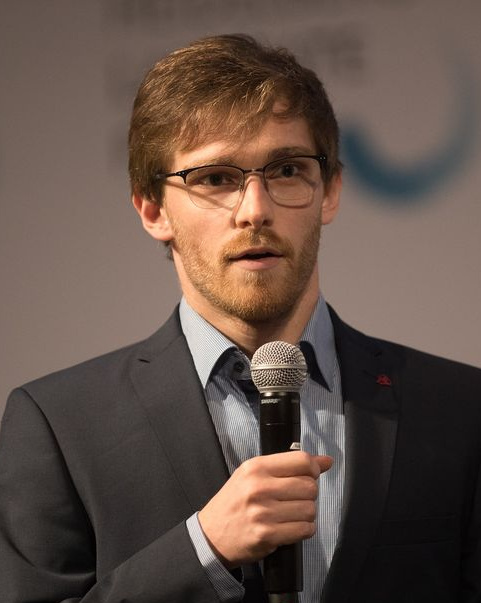
\includegraphics[height=2cm]{gfx/profilepicture}
						
					\footnotesize
					
					\underline{David}
					
					\underline{Stutz}
				\end{minipage}
				\begin{minipage}{0.225\textwidth}
					\centering
					
\includegraphics[height=2cm,trim={0.5cm 0 1.25cm 0}, clip]{gfx/nandhinichandramoorthy}
						
					\footnotesize
					
					Nandhini
					
					Chandramoorthy
				\end{minipage}
				\begin{minipage}{0.225\textwidth}
					\centering
					
\includegraphics[height=2cm,trim={0.1cm 0 0.15cm 0}, clip]{gfx/matthiashein}
					
					\footnotesize
					
					Matthias
					
					Hein
				\end{minipage}
				\begin{minipage}{0.225\textwidth}
					\centering
					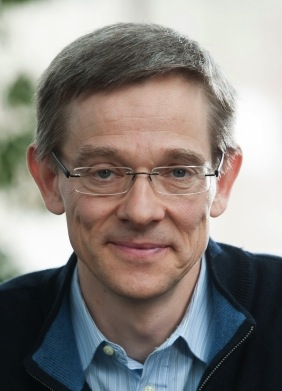
\includegraphics[height=2cm]{gfx/berntschiele}
					
					\footnotesize
					
					Bernt
					
					Schiele
				\end{minipage}
			\end{center}
			
			\begin{minipage}[t]{3.5cm}
				\vspace*{0px}
				\centering
				\begin{tikzpicture}
				\node at (0,0){
\includegraphics[height=1cm]{mpilogo-inf-narrow.eps}};
				\end{tikzpicture}
			\end{minipage}
			\hspace*{0.25cm}
			\begin{minipage}[t]{3.5cm}
				\vspace*{0px}
				\centering
				\begin{tikzpicture}
				\node at (0,0){
\includegraphics[height=1cm]{UT_WBMW_Rot_RGB.eps}};
				\end{tikzpicture}
			\end{minipage}
			\hspace*{0.5cm}
			\begin{minipage}[t]{3.5cm}
				\vspace*{0px}
				\centering
				\begin{tikzpicture}
				\node at (0,0){
\includegraphics[height=1cm]{IBM_logo_pos_RGB}};
				\end{tikzpicture}
			\end{minipage}
		\end{center}
	\end{frame}
	\endgroup
	
	\begin{frame}[t]{\bfseries\textit{1-Minute Overview}: Bit Error Robustness}
		\Large
		\vspace*{-0.75cm}
		
		\begin{minipage}[t]{0.5\textwidth}
			\vspace*{0cm}
			
			\begin{tcolorbox}[
				enhanced,
				boxsep=0pt,
				left=5pt,
				right=5pt,
				top=0pt,
				toptitle=4pt,
				bottomtitle=2pt,
				bottom=0pt,
				colback=white,
				colframe=gray!12!white,
				width=1\textwidth, 
				enlarge left by=0mm,
				arc=0pt,outer arc=0pt,
				boxrule=1pt,
				title=Random \textbf{bit errors}:,
				coltitle=MPIIblack,
				colbacktitle=gray!12!white,
				titlerule style=gray!12!white,
				collower=MPIIblack,
				]
				
				\vspace*{0.25cm}
				\hspace*{-0.2cm}
				\resizebox{!}{3.7cm}{
					\begin{tikzpicture}
					\begin{axis}[
							xmin=0.75,
							xmax=1,
							ymin=0,
							ymax=21,
							ymode=log,
							grid=both,
							grid style={line width=.1pt, draw=gray!25},
							major grid style={line width=.2pt,draw=gray!50},
							minor tick num=1,
							width=8cm,
							height=7cm,
							ytick={0.0001, 0.001, 0.01, 0.1, 1, 2.5, 10},
							yticklabels={$10^{-4}$, $10^{-3}$, $10^{-2}$, $10^{-1}$, $1$, $2.5$, $10$},
							xtick={0.79, 0.89, 0.99},
							xticklabel style={/pgf/number format/precision=2,/pgf/number format/fixed},
							scaled x ticks=false,
							yticklabel style={/pgf/number format/precision=2,/pgf/number format/fixed},
							scaled y ticks=false,
							ylabel=Bit Error Rate $p$ in \%,
							y label style={at={(axis description cs:0.025,0.5)},anchor=south,font=\large},
							xlabel={Supply Voltage, Normalized by $V_{\text{min}}$},
							x label style={at={(axis description cs:0.5,0.01)},anchor=north,font=\large},
						]
						
						\addplot[Error] coordinates {
							(0.75, 20.56)
							(0.792, 5.573)
							(0.833, 1.115)
							(0.875, 0.129)
							(0.917, 0.00686646)
							(0.958, 0.000190735)
							(1.0, 0)
						};\label{plot:error}
						\end{axis}
						\begin{axis}[
						axis y line*=right,
						xmin=0.75,
						xmax=1,
						ymax=1.03,
						ymin=0.48,
						xtick={},
						ytick={0.6, 0.8, 1},
						xticklabels={},
						width=8cm,
						height=7cm,
						ylabel=\begin{tabular}{c}Normalized Energy\\per SRAM Access\end{tabular},
						y label style={at={(axis description cs:1.3,0.5)},anchor=north,font=\large},
						legend style={fill=white, fill opacity=0.6, draw opacity=1,text opacity=1,at={(axis description cs:0.13,0.02)},anchor=south west,row sep=-2.5pt,font=\large,/tikz/every even column/.append style={row sep=0.5cm}},
						legend cell align={left},
						]
						\addlegendimage{/pgfplots/refstyle=plot:error}\addlegendentry{Bit Error Rate $p$};
						\addplot[Energy] coordinates {
							(0.75, 0.5625)
							(0.792, 0.626736111)
							(0.833, 0.694444444)
							(0.875, 0.765625)
							(0.917, 0.840277778)
							(0.958, 0.918402778)
							(1.0, 1)
						};
						\addlegendentry{Normalized Energy};
						\coordinate (Vmin) at (axis cs:1,0.485) {};
						\end{axis}
						%\node[anchor=north west,yshift=-0.4mm] at (Vmin){\small ${=}V_{\text{min}}$};
					\end{tikzpicture}
				}
			\end{tcolorbox}
		\end{minipage}
		\begin{minipage}[t]{0.45\textwidth}
			\vspace*{0cm}
			
		\end{minipage}
		\vspace*{-0.1cm}
	\end{frame}
	
	\begin{frame}[t]{\bfseries\textit{1-Minute Overview}: Bit Error Robustness}
		\Large
		\vspace*{-0.75cm}
		
		\begin{minipage}[t]{0.5\textwidth}
			\vspace*{0cm}
			
			\begin{tcolorbox}[
				enhanced,
				boxsep=0pt,
				left=5pt,
				right=5pt,
				top=0pt,
				toptitle=4pt,
				bottomtitle=2pt,
				bottom=0pt,
				colback=white,
				colframe=gray!12!white,
				width=1\textwidth, 
				enlarge left by=0mm,
				arc=0pt,outer arc=0pt,
				boxrule=1pt,
				title=Random \textbf{bit errors}:,
				coltitle=MPIIblack,
				colbacktitle=gray!12!white,
				titlerule style=gray!12!white,
				collower=MPIIblack,
				]
				
				\vspace*{0.25cm}
				\hspace*{-0.2cm}
				\resizebox{!}{3.7cm}{
					\begin{tikzpicture}
					\begin{axis}[
							xmin=0.75,
							xmax=1,
							ymin=0,
							ymax=21,
							ymode=log,
							grid=both,
							grid style={line width=.1pt, draw=gray!25},
							major grid style={line width=.2pt,draw=gray!50},
							minor tick num=1,
							width=8cm,
							height=7cm,
							ytick={0.0001, 0.001, 0.01, 0.1, 1, 2.5, 10},
							yticklabels={$10^{-4}$, $10^{-3}$, $10^{-2}$, $10^{-1}$, $1$, $2.5$, $10$},
							xtick={0.79, 0.89, 0.99},
							xticklabel style={/pgf/number format/precision=2,/pgf/number format/fixed},
							scaled x ticks=false,
							yticklabel style={/pgf/number format/precision=2,/pgf/number format/fixed},
							scaled y ticks=false,
							ylabel=Bit Error Rate $p$ in \%,
							y label style={at={(axis description cs:0.025,0.5)},anchor=south,font=\large},
							xlabel={Supply Voltage, Normalized by $V_{\text{min}}$},
							x label style={at={(axis description cs:0.5,0.01)},anchor=north,font=\large},
						]
						
						\addplot[Error] coordinates {
							(0.75, 20.56)
							(0.792, 5.573)
							(0.833, 1.115)
							(0.875, 0.129)
							(0.917, 0.00686646)
							(0.958, 0.000190735)
							(1.0, 0)
						};\label{plot:error}
						\end{axis}
						\begin{axis}[
						axis y line*=right,
						xmin=0.75,
						xmax=1,
						ymax=1.03,
						ymin=0.48,
						xtick={},
						ytick={0.6, 0.8, 1},
						xticklabels={},
						width=8cm,
						height=7cm,
						ylabel=\begin{tabular}{c}Normalized Energy\\per SRAM Access\end{tabular},
						y label style={at={(axis description cs:1.3,0.5)},anchor=north,font=\large},
						legend style={fill=white, fill opacity=0.6, draw opacity=1,text opacity=1,at={(axis description cs:0.13,0.02)},anchor=south west,row sep=-2.5pt,font=\large,/tikz/every even column/.append style={row sep=0.5cm}},
						legend cell align={left},
						]
						\addlegendimage{/pgfplots/refstyle=plot:error}\addlegendentry{Bit Error Rate $p$};
						\addplot[Energy] coordinates {
							(0.75, 0.5625)
							(0.792, 0.626736111)
							(0.833, 0.694444444)
							(0.875, 0.765625)
							(0.917, 0.840277778)
							(0.958, 0.918402778)
							(1.0, 1)
						};
						\addlegendentry{Normalized Energy};
						\coordinate (Vmin) at (axis cs:1,0.485) {};
						\end{axis}
					\end{tikzpicture}
				}
			\end{tcolorbox}
		\end{minipage}
		\begin{minipage}[t]{0.45\textwidth}
			\vspace*{0cm}
			
			\begin{tcolorbox}[
				enhanced,
				boxsep=0pt,
				left=5pt,
				right=5pt,
				top=0pt,
				toptitle=4pt,
				bottomtitle=2pt,
				bottom=0pt,
				colback=white,
				colframe=gray!12!white,
				width=1\textwidth, 
				enlarge left by=0mm,
				arc=0pt,outer arc=0pt,
				boxrule=1pt,
				title=Bit error \textbf{robustness}:,
				coltitle=MPIIblack,
				colbacktitle=gray!12!white,
				titlerule style=gray!12!white,
				collower=MPIIblack,
				]
			
				\vspace*{0.1cm}
				\hspace*{-0.1cm}
				\resizebox{!}{3.85cm}{
					\begin{tikzpicture}
					\begin{axis}[
							ymin=4.3,
							ymax=8,
							xmin=0,
							xmax=3,
							xtick={0, 0.01, 0.1, 0.5, 1, 2.5},
							xticklabels={$0$, $0.01$, $0.1$, $0.5$, $1$, $2.5$},
							ytick={4.3, 5, 6, 7, 8, 9, 10},
							scaled x ticks=false,
							xticklabel style={/pgf/number format/precision=2,/pgf/number format/fixed},
							scaled y ticks=false,
							yticklabel style={/pgf/number format/precision=2,/pgf/number format/fixed},
							log ticks with fixed point,
							grid=major,
							xlabel={Bit Error Rate $p$ in \%},
							ylabel={Robust Test Error RErr in \%},
							x label style={at={(axis description cs:0.5,0.02)},anchor=north,font=\large},
							y label style={at={(axis description cs:0.07,0.5)},anchor=south,font=\large},
							width=9cm,
							height=7cm,
							title={\hspace*{2.75cm}CIFAR-10},
							title style={at={(axis description cs:0.5, 0.95)},anchor=south},
						]
						
						\addplot[OptNormal] coordinates {
						(0.0, 4.36) % 0.0
						(0.005, 4.71) % 0.005
						(0.01, 4.82) % 0.01
						(0.025, 5.09) % 0.025
						(0.05, 5.510000000000001) % 0.05
						(0.075, 5.949999999999999) % 0.075
						(0.1, 6.370000000000001) % 0.1
						(0.25, 10.190000000000001) % 0.25
						(0.5, 24.759999999999998) % 0.5
						(0.75, 50.1) % 0.75
						(1.0, 72.65) % 1.0
						(1.5, 87.4) % 1.5
						(2.0, 89.75999999999999) % 2.0
						(2.5, 90.14999999999999) % 2.5
						};
						\label{normal1}
						\addplot[OptQuant] coordinates {
						(0.0, 4.32)
						(0.005, 4.52)
						(0.01, 4.6)
						(0.025, 4.83)
						(0.05, 5.1)
						(0.075, 5.3100000000000005)
						(0.1, 5.54)
						(0.25, 7.08)
						(0.5, 11.28)
						(0.75, 18.44)
						(1.0, 32.05)
						(1.5, 68.65)
						(2.0, 85.28)
						(2.5, 89.01)
						};
						\label{quant1}
						\addplot[OptClipping] coordinates {
						(0.0, 4.42)
						(0.005, 4.569999999999999)
						(0.01, 4.66)
						(0.025, 4.81)
						(0.05, 5.01)
						(0.075, 5.16)
						(0.1, 5.3100000000000005)
						(0.25, 6.17)
						(0.5, 6.529999999999999)
						(0.75, 6.8500000000000005)
						(1.0, 7.180000000000001)
						(1.5, 7.920000000000001)
						(2.0, 8.7)
						(2.5, 9.02)
						};
						\label{clipping1}
						\addplot[OptRandom] coordinates {
						(0.0, 4.44)
						(0.005, 4.65)
						(0.01, 4.67)
						(0.025, 4.8500000000000005)
						(0.05, 5.07)
						(0.075, 5.24)
						(0.1, 5.37)
						(0.25, 5.81)
						(0.5, 6.18)
						(0.75, 6.47)
						(1.0, 6.710000000000001)
						(1.5, 7.13)
						(2.0, 7.580000000000001)
						(2.5, 8.02)
						};
						\label{random1}
						\coordinate (e) at (axis cs:0.5,6.18);
						\coordinate (e2) at (axis cs:0.1,5.37);
						\end{axis}
						\draw[colorbrewer1,line width=2pt] (e) circle (6pt);
						\draw[colorbrewer1,line width=2pt,-] ($(e) - (0,0.2)$) -- ($(e) - (0,2.9)$);
						\draw[colorbrewer1,line width=2pt,-] ($(e) - (0.2,0)$) -- ($(e) - (6,0)$);
						\node[opacity=1,fill opacity=0.75,fill=white,inner sep=0] at ($(e) - (3.65,0)$){\bfseries\color{colorbrewer1}$\mathbf{6.18\%}{\approx}\mathbf{30\%}$ reduction};
						
						\draw[colorbrewer1,line width=2pt] (e2) circle (6pt);
						\draw[colorbrewer1,line width=2pt,-] ($(e2) - (0,0.2)$) -- ($(e2) - (0,1.7)$);
						\draw[colorbrewer1,line width=2pt,-] ($(e2) - (0.2,0)$) -- ($(e2) - (4.7,0)$);
						\node[opacity=1,fill opacity=0.75,fill=white,inner sep=0] at ($(e2) - (2.35,0)$){\bfseries\color{colorbrewer1}$\mathbf{5.37\%}{\approx}\mathbf{20\%}$ reduction};
						
						\node [draw,fill=white,text opacity=1,fill opacity=0.85,anchor=north west] at (rel axis cs: 0.02, 1.1) {\shortstack[l]{
						\underline{$8$ Bit Quant.:}\\
						\ref{normal1} \textsc{Normal}\\[1px]
						\ref{quant1} \textsc{RQuant}\\ 
						\ref{clipping1} +\textsc{Clipping}\\[1px]
						\ref{random1} +\textsc{RandBET}}};
					\end{tikzpicture}
				}
			\end{tcolorbox}
		\end{minipage}
		\vspace*{-0.1cm}
	\end{frame}
	
	\begin{frame}[t]{\bfseries\textit{1-Minute Overview}: Bit Error Robustness}
		\Large
		\vspace*{-0.75cm}
		
		\begin{minipage}[t]{0.5\textwidth}
			\vspace*{0cm}
			
			\begin{tcolorbox}[
				enhanced,
				boxsep=0pt,
				left=5pt,
				right=5pt,
				top=0pt,
				toptitle=4pt,
				bottomtitle=2pt,
				bottom=0pt,
				colback=white,
				colframe=gray!12!white,
				width=1\textwidth, 
				enlarge left by=0mm,
				arc=0pt,outer arc=0pt,
				boxrule=1pt,
				title=Random \textbf{bit errors}:,
				coltitle=MPIIblack,
				colbacktitle=gray!12!white,
				titlerule style=gray!12!white,
				collower=MPIIblack,
				]
				
				\vspace*{0.25cm}
				\hspace*{-0.2cm}
				\resizebox{!}{3.7cm}{
					\begin{tikzpicture}
					\begin{axis}[
							xmin=0.75,
							xmax=1,
							ymin=0,
							ymax=21,
							ymode=log,
							grid=both,
							grid style={line width=.1pt, draw=gray!25},
							major grid style={line width=.2pt,draw=gray!50},
							minor tick num=1,
							width=8cm,
							height=7cm,
							ytick={0.0001, 0.001, 0.01, 0.1, 1, 2.5, 10},
							yticklabels={$10^{-4}$, $10^{-3}$, $10^{-2}$, $10^{-1}$, $1$, $2.5$, $10$},
							xtick={0.79, 0.89, 0.99},
							xticklabel style={/pgf/number format/precision=2,/pgf/number format/fixed},
							scaled x ticks=false,
							yticklabel style={/pgf/number format/precision=2,/pgf/number format/fixed},
							scaled y ticks=false,
							ylabel=Bit Error Rate $p$ in \%,
							y label style={at={(axis description cs:0.025,0.5)},anchor=south,font=\large},
							xlabel={Supply Voltage, Normalized by $V_{\text{min}}$},
							x label style={at={(axis description cs:0.5,0.01)},anchor=north,font=\large},
						]
						
						\addplot[Error] coordinates {
							(0.75, 20.56)
							(0.792, 5.573)
							(0.833, 1.115)
							(0.875, 0.129)
							(0.917, 0.00686646)
							(0.958, 0.000190735)
							(1.0, 0)
						};\label{plot:error}
						\end{axis}
						\begin{axis}[
						axis y line*=right,
						xmin=0.75,
						xmax=1,
						ymax=1.03,
						ymin=0.48,
						xtick={},
						ytick={0.6, 0.8, 1},
						xticklabels={},
						width=8cm,
						height=7cm,
						ylabel=\begin{tabular}{c}Normalized Energy\\per SRAM Access\end{tabular},
						y label style={at={(axis description cs:1.3,0.5)},anchor=north,font=\large},
						legend style={fill=white, fill opacity=0.6, draw opacity=1,text opacity=1,at={(axis description cs:0.13,0.02)},anchor=south west,row sep=-2.5pt,font=\large,/tikz/every even column/.append style={row sep=0.5cm}},
						legend cell align={left},
						]
						\addlegendimage{/pgfplots/refstyle=plot:error}\addlegendentry{Bit Error Rate $p$};
						\addplot[Energy] coordinates {
							(0.75, 0.5625)
							(0.792, 0.626736111)
							(0.833, 0.694444444)
							(0.875, 0.765625)
							(0.917, 0.840277778)
							(0.958, 0.918402778)
							(1.0, 1)
						};
						\addlegendentry{Normalized Energy};
						\coordinate (Vmin) at (axis cs:1,0.485) {};
						\end{axis}
						%\node[anchor=north west,yshift=-0.4mm] at (Vmin){\small ${=}V_{\text{min}}$};
					\end{tikzpicture}
				}
			\end{tcolorbox}
		\end{minipage}
		\begin{minipage}[t]{0.45\textwidth}
			\vspace*{0cm}
			
			\begin{tcolorbox}[
				enhanced,
				boxsep=0pt,
				left=5pt,
				right=5pt,
				top=0pt,
				toptitle=4pt,
				bottomtitle=2pt,
				bottom=0pt,
				colback=white,
				colframe=gray!12!white,
				width=1\textwidth, 
				enlarge left by=0mm,
				arc=0pt,outer arc=0pt,
				boxrule=1pt,
				title=Bit error \textbf{robustness}:,
				coltitle=MPIIblack,
				colbacktitle=gray!12!white,
				titlerule style=gray!12!white,
				collower=MPIIblack,
				]
			
				\vspace*{0.1cm}
				\hspace*{-0.1cm}
				\resizebox{!}{3.85cm}{
					\begin{tikzpicture}
					\begin{axis}[
							ymin=4.3,
							ymax=8,
							xmin=0,
							xmax=3,
							xtick={0, 0.01, 0.1, 0.5, 1, 2.5},
							xticklabels={$0$, $0.01$, $0.1$, $0.5$, $1$, $2.5$},
							ytick={4.3, 5, 6, 7, 8, 9, 10},
							scaled x ticks=false,
							xticklabel style={/pgf/number format/precision=2,/pgf/number format/fixed},
							scaled y ticks=false,
							yticklabel style={/pgf/number format/precision=2,/pgf/number format/fixed},
							log ticks with fixed point,
							grid=major,
							xlabel={Bit Error Rate $p$ in \%},
							ylabel={Robust Test Error RErr in \%},
							x label style={at={(axis description cs:0.5,0.02)},anchor=north,font=\large},
							y label style={at={(axis description cs:0.07,0.5)},anchor=south,font=\large},
							width=9cm,
							height=7cm,
							title={\hspace*{2.75cm}CIFAR-10},
							title style={at={(axis description cs:0.5, 0.95)},anchor=south},
						]
						
						\addplot[OptNormal] coordinates {
						(0.0, 4.36) % 0.0
						(0.005, 4.71) % 0.005
						(0.01, 4.82) % 0.01
						(0.025, 5.09) % 0.025
						(0.05, 5.510000000000001) % 0.05
						(0.075, 5.949999999999999) % 0.075
						(0.1, 6.370000000000001) % 0.1
						(0.25, 10.190000000000001) % 0.25
						(0.5, 24.759999999999998) % 0.5
						(0.75, 50.1) % 0.75
						(1.0, 72.65) % 1.0
						(1.5, 87.4) % 1.5
						(2.0, 89.75999999999999) % 2.0
						(2.5, 90.14999999999999) % 2.5
						};
						\label{normal1}
						\addplot[OptQuant] coordinates {
						(0.0, 4.32)
						(0.005, 4.52)
						(0.01, 4.6)
						(0.025, 4.83)
						(0.05, 5.1)
						(0.075, 5.3100000000000005)
						(0.1, 5.54)
						(0.25, 7.08)
						(0.5, 11.28)
						(0.75, 18.44)
						(1.0, 32.05)
						(1.5, 68.65)
						(2.0, 85.28)
						(2.5, 89.01)
						};
						\label{quant1}
						\addplot[OptClipping] coordinates {
						(0.0, 4.42)
						(0.005, 4.569999999999999)
						(0.01, 4.66)
						(0.025, 4.81)
						(0.05, 5.01)
						(0.075, 5.16)
						(0.1, 5.3100000000000005)
						(0.25, 6.17)
						(0.5, 6.529999999999999)
						(0.75, 6.8500000000000005)
						(1.0, 7.180000000000001)
						(1.5, 7.920000000000001)
						(2.0, 8.7)
						(2.5, 9.02)
						};
						\label{clipping1}
						\addplot[OptRandom] coordinates {
						(0.0, 4.44)
						(0.005, 4.65)
						(0.01, 4.67)
						(0.025, 4.8500000000000005)
						(0.05, 5.07)
						(0.075, 5.24)
						(0.1, 5.37)
						(0.25, 5.81)
						(0.5, 6.18)
						(0.75, 6.47)
						(1.0, 6.710000000000001)
						(1.5, 7.13)
						(2.0, 7.580000000000001)
						(2.5, 8.02)
						};
						\label{random1}
						\coordinate (e) at (axis cs:0.5,6.18);
						\coordinate (e2) at (axis cs:0.1,5.37);
						\end{axis}
						\draw[colorbrewer1,line width=2pt] (e) circle (6pt);
						\draw[colorbrewer1,line width=2pt,-] ($(e) - (0,0.2)$) -- ($(e) - (0,2.9)$);
						\draw[colorbrewer1,line width=2pt,-] ($(e) - (0.2,0)$) -- ($(e) - (6,0)$);
						\node[opacity=1,fill opacity=0.75,fill=white,inner sep=0] at ($(e) - (3.65,0)$){\bfseries\color{colorbrewer1}$\mathbf{6.18\%}{\approx}\mathbf{30\%}$ reduction};
						
						\draw[colorbrewer1,line width=2pt] (e2) circle (6pt);
						\draw[colorbrewer1,line width=2pt,-] ($(e2) - (0,0.2)$) -- ($(e2) - (0,1.7)$);
						\draw[colorbrewer1,line width=2pt,-] ($(e2) - (0.2,0)$) -- ($(e2) - (4.7,0)$);
						\node[opacity=1,fill opacity=0.75,fill=white,inner sep=0] at ($(e2) - (2.35,0)$){\bfseries\color{colorbrewer1}$\mathbf{5.37\%}{\approx}\mathbf{20\%}$ reduction};
						
						\node [draw,fill=white,text opacity=1,fill opacity=0.85,anchor=north west] at (rel axis cs: 0.02, 1.1) {\shortstack[l]{
						\underline{$8$ Bit Quant.:}\\
						\ref{normal1} \textsc{Normal}\\[1px]
						\ref{quant1} \textsc{RQuant}\\ 
						\ref{clipping1} +\textsc{Clipping}\\[1px]
						\ref{random1} +\textsc{RandBET}}};
					\end{tikzpicture}
				}
			\end{tcolorbox}
		\end{minipage}
		\vspace*{-0.1cm}
		
		\begin{tcolorbox}[
			enhanced,
			boxsep=4pt,
			left=0pt,
			right=0pt,
			top=2pt,
			toptitle=0pt,
			bottomtitle=2pt,
			bottom=0pt,
			colback=gray!12!white,
			colframe=gray!12!white,
			width=1\textwidth, 
			enlarge left by=0mm,
			arc=0pt,outer arc=0pt,
			boxrule=1pt,
			title=\bfseries More details:,
			coltitle=MPIIblack,
			colbacktitle=gray!12!white,
			titlerule style=white,
			collower=MPIIblack,
			]
			\color{MPIIblack}
			Paper \& code: \href{http://davidstutz.de/ccat}{\texttt{davidstutz.de/randbet}}\\
			Contact: \texttt{david.stutz@mpi-inf.mpg.de}
		\end{tcolorbox}
	\end{frame}
	
	\begin{frame}[t]{\bfseries Interested?}
		\Large 
		\begin{tcolorbox}[
			enhanced,
			boxsep=4pt,
			left=0pt,
			right=0pt,
			top=2pt,
			toptitle=0pt,
			bottomtitle=2pt,
			bottom=0pt,
			colback=gray!12!white,
			colframe=gray!12!white,
			width=1\textwidth, 
			enlarge left by=0mm,
			arc=0pt,outer arc=0pt,
			boxrule=1pt,
			title=\bfseries More details:,
			coltitle=MPIIblack,
			colbacktitle=gray!12!white,
			titlerule style=white,
			collower=MPIIblack,
			]
			\color{MPIIblack}
			Paper \& code: \href{http://davidstutz.de/ccat}{\texttt{davidstutz.de/randbet}}\\
			Contact: \texttt{david.stutz@mpi-inf.mpg.de}
		\end{tcolorbox}
		
		\textbf{Outline:}
		\vspace*{0.35cm}
		
		\hspace*{0.25cm}\begin{minipage}{\textwidth}
			\begin{enumerate}
				\item Bit errors in DNN accelerators
				\item Error model and contributions
				\item Robust quantization, weight clipping, and \\random bit error training
				\item Results and energy savings
			\end{enumerate}
		\end{minipage}
	\end{frame}
	
	\begin{frame}[t]{\bfseries {\color{colorbrewer5}Energy Consumption} in DNN Accelerators}
		\vspace*{0.55cm}
		\centering
		\hspace*{1.3cm}
		\begin{tikzpicture}
		\begin{axis}[
				xmin=0.75,
				xmax=1,
				axis y line*=right,
				ymax=1.03,
				ymin=0.48,
				xtick={},
				ytick={0.6, 0.8, 1},
				grid=both,
				grid style={line width=.1pt, draw=gray!25},
				major grid style={line width=.2pt,draw=gray!50},
				minor tick num=1,
				width=10cm,
				height=7cm,
				xticklabel style={/pgf/number format/precision=2,/pgf/number format/fixed},
				scaled x ticks=false,
				yticklabel style={/pgf/number format/precision=2,/pgf/number format/fixed},
				scaled y ticks=false,
				ylabel=\begin{tabular}{c}Normalized Energy\\per SRAM Access\end{tabular},
				y label style={at={(axis description cs:1.225,0.5)},anchor=north,font=\large},
				legend style={fill=white, fill opacity=0.6, draw opacity=1,text opacity=1,at={(axis description cs:0.13,0.02)},anchor=south west,row sep=-2.5pt,font=\large,/tikz/every even column/.append style={row sep=0.5cm}},
				legend cell align={left},
				xlabel={Supply Voltage, Normalized by {\color{colorbrewer1}$\mathbf{V_{\text{min}}}$}},
				x label style={at={(axis description cs:0.5,0.02)},anchor=north,font=\large},
			]
			
			\addplot[Energy] coordinates {
				(0.75, 0.5625)
				(0.792, 0.626736111)
				(0.833, 0.694444444)
				(0.875, 0.765625)
				(0.917, 0.840277778)
				(0.958, 0.918402778)
				(1.0, 1)
			};
			\addlegendentry{Normalized Energy};
			\coordinate (Vmin) at (axis cs:1,0.485) {};
			\end{axis}
			\node[anchor=north west,yshift=-0.4mm] at (Vmin){\small\color{colorbrewer1} ${=}V_{\text{min}}$};
			\begin{axis}[
				xmin=0.75,
				xmax=1,
				ymin=0,
				ymax=21,
				ymode=log,
				grid=both,
				grid style={line width=.1pt, draw=gray!25},
				major grid style={line width=.2pt,draw=gray!50},
				minor tick num=1,
				width=10cm,
				height=7cm,
				ytick={0.0001, 0.001, 0.01, 0.1, 1, 2.5, 10, 20},
				yticklabels={$10^{-4}$, $10^{-3}$, $10^{-2}$, $10^{-1}$, 1, \raisebox{2px}{2.5}, \raisebox{-8px}{10}, \raisebox{4px}{20}},
				xticklabel style={/pgf/number format/precision=2,/pgf/number format/fixed},
				scaled x ticks=false,
				yticklabel style={/pgf/number format/precision=2,/pgf/number format/fixed},
				scaled y ticks=false,
				ticks=none,
			]
			
			\addplot[Error,transparent] coordinates {
				(0.75, 20.56)
				(0.792, 5.573)
				(0.833, 1.115)
				(0.875, 0.129)
				(0.917, 0.00686646)
				(0.958, 0.000190735)
				(1.0, 0)
			};
			\end{axis}
		\end{tikzpicture}
	\end{frame}
	
	\begin{frame}[t]{\bfseries {\color{colorbrewer5}Energy Consumption} in DNN Accelerators}
		\vspace*{0.55cm}
		\centering
		\hspace*{0.275cm}
		\begin{tikzpicture}
		\begin{axis}[
				xmin=0.75,
				xmax=1,
				axis y line*=right,
				ymax=1.03,
				ymin=0.48,
				xtick={},
				ytick={0.6, 0.8, 1},
				grid=both,
				grid style={line width=.1pt, draw=gray!25},
				major grid style={line width=.2pt,draw=gray!50},
				minor tick num=1,
				width=10cm,
				height=7cm,
				xticklabel style={/pgf/number format/precision=2,/pgf/number format/fixed,font=\small},
				scaled x ticks=false,
				yticklabel style={/pgf/number format/precision=2,/pgf/number format/fixed,font=\small},
				scaled y ticks=false,
				ylabel=\begin{tabular}{c}Normalized Energy\\per SRAM Access\end{tabular},
				y label style={at={(axis description cs:1.225,0.5)},anchor=north,font=\large},
				legend style={fill=white, fill opacity=0.6, draw opacity=1,text opacity=1,at={(axis description cs:0.13,0.02)},anchor=south west,row sep=-2.5pt,font=\large,/tikz/every even column/.append style={row sep=0.5cm}},
				legend cell align={left},
				xlabel={Supply Voltage, Normalized by {$V_{\text{min}}$}},
				x label style={at={(axis description cs:0.5,0.02)},anchor=north,font=\large},
			]
			
			\addplot[Energy] coordinates {
				(0.75, 0.5625)
				(0.792, 0.626736111)
				(0.833, 0.694444444)
				(0.875, 0.765625)
				(0.917, 0.840277778)
				(0.958, 0.918402778)
				(1.0, 1)
			};
			\addlegendentry{Normalized Energy};
			\coordinate (Vmin) at (axis cs:1,0.485) {};
			\coordinate (v2) at (axis cs:0.833, 0.694444444) {};
			\coordinate (v3) at (axis cs:0.875, 0.765625) {};
			\end{axis}
			\begin{axis}[
				xmin=0.75,
				xmax=1,
				ymin=0,
				ymax=21,
				ymode=log,
				grid=both,
				grid style={line width=.1pt, draw=gray!25},
				major grid style={line width=.2pt,draw=gray!50},
				minor tick num=1,
				width=10cm,
				height=7cm,
				ytick={0.0001, 0.001, 0.01, 0.1, 1, 2.5, 10, 20},
				yticklabels={$10^{-4}$, $10^{-3}$, $10^{-2}$, $10^{-1}$, 1, \raisebox{2px}{2.5}, \raisebox{-8px}{10}, \raisebox{4px}{20}},
				xticklabel style={/pgf/number format/precision=2,/pgf/number format/fixed},
				scaled x ticks=false,
				yticklabel style={/pgf/number format/precision=2,/pgf/number format/fixed},
				scaled y ticks=false,
				ticks=none,
			]
			
			\addplot[Error,transparent] coordinates {
				(0.75, 20.56)
				(0.792, 5.573)
				(0.833, 1.115)
				(0.875, 0.129)
				(0.917, 0.00686646)
				(0.958, 0.000190735)
				(1.0, 0)
			};
			\end{axis}
			\node[anchor=north west,yshift=-0.4mm] at (Vmin){\small ${=}V_{\text{min}}$};
			\node[anchor=south east,draw=black,inner sep=0.25pt,line width=1pt,xshift=-0.15cm] at (v2) {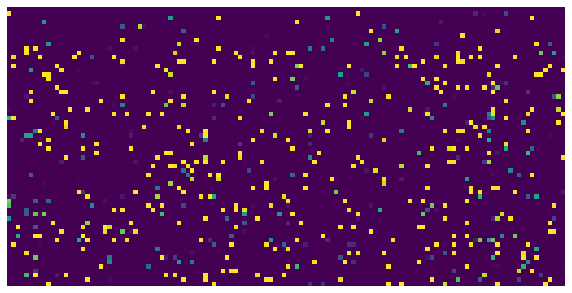
\includegraphics[height=2cm]{gfx/18_2}};
			\node[anchor=north west,draw=black,inner sep=0.25pt,line width=1pt,xshift=0.15cm] at (v3) {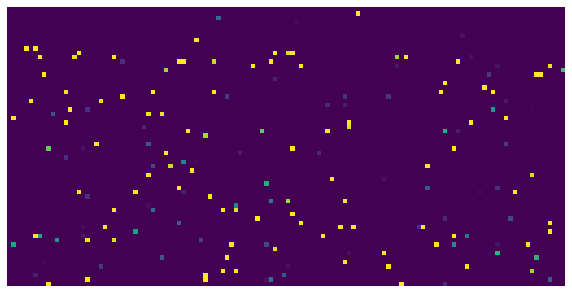
\includegraphics[height=2cm]{gfx/18_3}};
			\draw[line width=1pt] (v2) circle(3pt);
			\draw[-,line width=1pt] ($(v2) + (0,0.1)$) -- ($(v2) + (0,1.05)$) -- ($(v2) + (-0.175,1.05)$);
			\draw[line width=1pt] (v3) circle(3pt);
			\draw[-,line width=1pt] ($(v3) + (0,-0.1)$) -- ($(v3) - (0,1.05)$) -- ($(v3) - (-0.175,1.05)$);
		\end{tikzpicture}
	\end{frame}

	\begin{frame}[t]{\bfseries Low-Voltage Operation and {\color{colorbrewer2}Bit Errors}}
		\vspace*{0.25cm}
		\centering
		\begin{tikzpicture}
		\begin{axis}[
				xmin=0.75,
				xmax=1,
				ymin=0,
				ymax=21,
				ymode=log,
				grid=both,
				grid style={line width=.1pt, draw=gray!25},
				major grid style={line width=.2pt,draw=gray!50},
				minor tick num=1,
				width=10cm,
				height=7cm,
				ytick={0.0001, 0.001, 0.01, 0.1, 1, 2.5, 10, 20},
				yticklabels={$10^{-4}$, $10^{-3}$, $10^{-2}$, $10^{-1}$, 1, \raisebox{2px}{2.5}, \raisebox{-8px}{10}, \raisebox{4px}{20}},
				xticklabel style={/pgf/number format/precision=2,/pgf/number format/fixed},
				scaled x ticks=false,
				yticklabel style={/pgf/number format/precision=2,/pgf/number format/fixed},
				scaled y ticks=false,
				ylabel=Bit Error Rate $p$ in \%,
				y label style={at={(axis description cs:0.05,0.5)},anchor=south,font=\large},
				xlabel={Supply Voltage, Normalized by $V_{\text{min}}$},
				x label style={at={(axis description cs:0.5,0.02)},anchor=north,font=\large},
			]
			
			\addplot[Error] coordinates {
				(0.75, 20.56)
				(0.792, 5.573)
				(0.833, 1.115)
				(0.875, 0.129)
				(0.917, 0.00686646)
				(0.958, 0.000190735)
				(1.0, 0)
			};\label{plot:error}
			\end{axis}
			\begin{axis}[
			axis y line*=right,
			xmin=0.75,
			xmax=1,
			ymax=1.03,
			ymin=0.48,
			xtick={},
			ytick={0.6, 0.8, 1},
			xticklabels={},
			width=10cm,
			height=7cm,
			ylabel=\begin{tabular}{c}Normalized Energy\\per SRAM Access\end{tabular},
			y label style={at={(axis description cs:1.225,0.5)},anchor=north,font=\large},
			legend style={fill=white, fill opacity=0.6, draw opacity=1,text opacity=1,at={(axis description cs:0.13,0.02)},anchor=south west,row sep=-2.5pt,font=\large,/tikz/every even column/.append style={row sep=0.5cm}},
			legend cell align={left},
			]
			\addlegendimage{/pgfplots/refstyle=plot:error}\addlegendentry{Bit Error Rate $p$};
			\addplot[Energy] coordinates {
				(0.75, 0.5625)
				(0.792, 0.626736111)
				(0.833, 0.694444444)
				(0.875, 0.765625)
				(0.917, 0.840277778)
				(0.958, 0.918402778)
				(1.0, 1)
			};
			\addlegendentry{Normalized Energy};
			\coordinate (Vmin) at (axis cs:1,0.485) {};
			\end{axis}
			\node[anchor=north west,yshift=-0.4mm] at (Vmin){\small ${=}V_{\text{min}}$};
		\end{tikzpicture}
	\end{frame}
	
	\begin{frame}[t]{\bfseries Bit Error Impact on DNNs on CIFAR-10}
		\vspace*{0.25cm}
		\centering
		\hspace*{-1.6cm}
		\begin{tikzpicture}[overlay,remember picture]
			\draw[line width=1pt,arrow,colorbrewer1] (10.5, 8)[out=325,in=45] to (10.5, 6);
			\node[colorbrewer1,fill=white,text opacity=1,fill opacity=1] at (10.5, 7) {Axis Changed!};
		\end{tikzpicture}
		\begin{tikzpicture}
		\begin{axis}[
				ymin=4.3,
				ymax=8,
				xmin=0,
				xmax=3,
				xtick={0, 0.01, 0.05, 0.1, 0.5, 1, 2.5},
				xticklabels={$0$, $0.01$, $0.05$, $0.1$, $0.5$, $1$, $2.5$},
				ytick={4.3, 5, 6, 7, 8, 9, 10},
				scaled x ticks=false,
				xticklabel style={/pgf/number format/precision=2,/pgf/number format/fixed},
				scaled y ticks=false,
				yticklabel style={/pgf/number format/precision=2,/pgf/number format/fixed},
				log ticks with fixed point,
				grid=major,
				xlabel={Bit Error Rate $p$ in \%},
				ylabel={Robust Test Error RErr in \%},
				x label style={at={(axis description cs:0.5,0.02)},anchor=north,font=\large},
				y label style={at={(axis description cs:0.07,0.5)},anchor=south,font=\large},
				width=10cm,
				height=7cm,
				legend style={at={(axis description cs:0.02,0.98)},anchor=north west,font=\small,fill opacity=0.4,text opacity=1},
				legend cell align={left},
			]
			
			\addplot[OptNormal] coordinates {
			(0.0, 4.36) % 0.0
			(0.005, 4.71) % 0.005
			(0.01, 4.82) % 0.01
			(0.025, 5.09) % 0.025
			(0.05, 5.510000000000001) % 0.05
			(0.075, 5.949999999999999) % 0.075
			(0.1, 6.370000000000001) % 0.1
			(0.25, 10.190000000000001) % 0.25
			(0.5, 24.759999999999998) % 0.5
			(0.75, 50.1) % 0.75
			(1.0, 72.65) % 1.0
			(1.5, 87.4) % 1.5
			(2.0, 89.75999999999999) % 2.0
			(2.5, 90.14999999999999) % 2.5
			};
			\label{normal1}
			\end{axis}
			\node [draw,fill=white,text opacity=1,fill opacity=0.85,anchor=north west] at (rel axis cs: 0.02, 0.98) {\shortstack[l]{
			\underline{$8$ Bit Quant. CIFAR-10:}\\
			\ref{normal1} \textsc{Normal}}};
		\end{tikzpicture}
	\end{frame}
	
	\begin{frame}[t]{\bfseries Bit Error Model and Contributions}
		\Large 
		
		\underline{Bit error model:}
		\vspace*{1.25cm}
		
		\begin{tikzpicture}[remember picture,overlay]
			\node[anchor=north west] at (-0.25,1.75){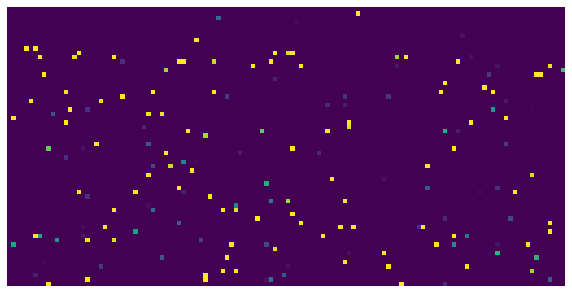
\includegraphics[width=6cm,trim={0 5cm 0 0},clip]{gfx/18_3}};
			\node[anchor=north west] at (5.75,1.75){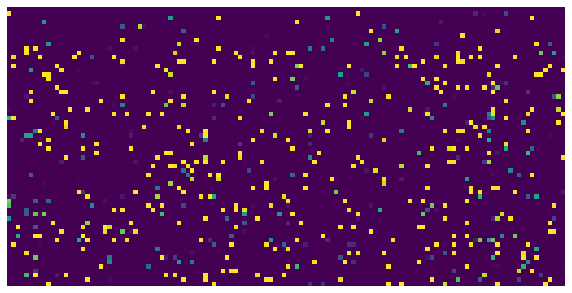
\includegraphics[width=6cm,trim={0 5cm 0 0},clip]{gfx/18_2}};
			\draw[line width=1pt,-] (2.75,-0.175) -- (2.75,-0.5) -- (4.5,-0.5);
			\draw[line width=1pt,-] (7,-0.5) -- (8.75,-0.5) -- (8.75,-0.175);
			\node at (5.75,-0.5){\normalsize subset of};
			\node[anchor=north west,fill=white,fill opacity=0.6,text opacity=1,inner sep=2.5pt] at (0.1, 1.4){\normalsize $p{\approx}0.86\%$};
			\node[anchor=north west,fill=white,fill opacity=0.6,text opacity=1,inner sep=2.5pt] at (6.1, 1.4){\normalsize $p{\approx}2.75\%$};
		\end{tikzpicture}
		
		\vspace*{0.5cm}
		\begin{itemize}
			\item Uniform (across locations+chips) random bit errors.
		\end{itemize}
	\end{frame}
	
	\begin{frame}[t]{\bfseries Bit Error Model and Contributions}
		\Large 
		
		\underline{Bit error model:}
		\vspace*{1.25cm}
		
		\begin{tikzpicture}[remember picture,overlay]
			\node[anchor=north west] at (-0.25,1.75){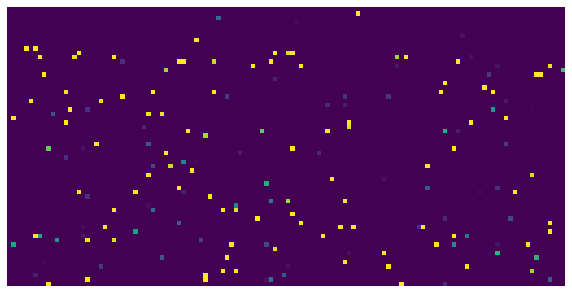
\includegraphics[width=6cm,trim={0 5cm 0 0},clip]{gfx/18_3}};
			\node[anchor=north west] at (5.75,1.75){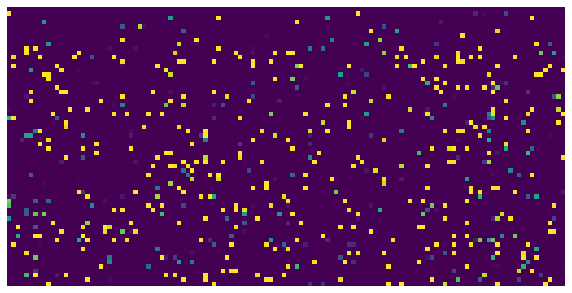
\includegraphics[width=6cm,trim={0 5cm 0 0},clip]{gfx/18_2}};
			\draw[line width=1pt,-] (2.75,-0.175) -- (2.75,-0.5) -- (4.5,-0.5);
			\draw[line width=1pt,-] (7,-0.5) -- (8.75,-0.5) -- (8.75,-0.175);
			\node at (5.75,-0.5){\normalsize subset of};
			\node[anchor=north west,fill=white,fill opacity=0.6,text opacity=1,inner sep=2.5pt] at (0.1, 1.4){\normalsize $p{\approx}0.86\%$};
			\node[anchor=north west,fill=white,fill opacity=0.6,text opacity=1,inner sep=2.5pt] at (6.1, 1.4){\normalsize $p{\approx}2.75\%$};
		\end{tikzpicture}
		
		\vspace*{0.5cm}
		\begin{itemize}
			\item Uniform (across locations+chips) random bit errors.
		\end{itemize}
		
		\vspace*{0.2cm}
		\underline{Contributions:}
		\begin{itemize}
			\item Robust fixed-point quantization (\textsc{RQuant}).
			\item Weight clipping as regularization (\textsc{Clipping}).
			\item Random bit error training (\textsc{RandBET}).
		\end{itemize}
	\end{frame}
	
	\begin{frame}[t]{\bfseries Robust Quantization (\textsc{RQuant})}
		\Large
		
		Simple fixed-point quantization scheme:
		\begin{align*}
			Q(w_i) = \left\lfloor\frac{w_i}{\Delta}\right\rfloor, Q^{-1}(v_i) = \Delta v_i, \Delta = \frac{q_{\text{max}}}{w^{m - 1} - 1}\notag
		\end{align*}
		\vspace*{-0.5cm}
		\begin{itemize}
			\item weight $w_i \in [-q_{\text{max}}, q_{\text{max}}]$, $m$ bits (\eg, $m = 8$)
		\end{itemize}
		\vspace*{0.15cm}
	\end{frame}
	
	\begin{frame}[t]{\bfseries Robust Quantization (\textsc{RQuant})}
		\Large
		
		Simple fixed-point quantization scheme:
		\begin{align*}
			Q(w_i) = \left\lfloor\frac{w_i}{\Delta}\right\rfloor, Q^{-1}(v_i) = \Delta v_i, \Delta = \frac{q_{\text{max}}}{w^{m - 1} - 1}\notag
		\end{align*}
		\vspace*{-0.5cm}
		\begin{itemize}
			\item weight $w_i \in [-q_{\text{max}}, q_{\text{max}}]$, $m$ bits (\eg, $m = 8$)
		\end{itemize}
		\vspace*{0.15cm}
		\begin{tcolorbox}[
			enhanced,
			boxsep=0pt,
			left=5pt,
			right=5pt,
			top=0pt,
			toptitle=4pt,
			bottomtitle=2pt,
			bottom=0pt,
			colback=white,
			colframe=gray!12!white,
			width=1\textwidth, 
			enlarge left by=0mm,
			arc=0pt,outer arc=0pt,
			boxrule=1pt,
			title=,
			coltitle=MPIIblack,
			colbacktitle=gray!12!white,
			titlerule style=gray!12!white,
			collower=MPIIblack,
			]
			\begin{center}
				\resizebox{\textwidth}{!}{
					\begin{tikzpicture}
						\node[anchor=north west] at (-0.25,0){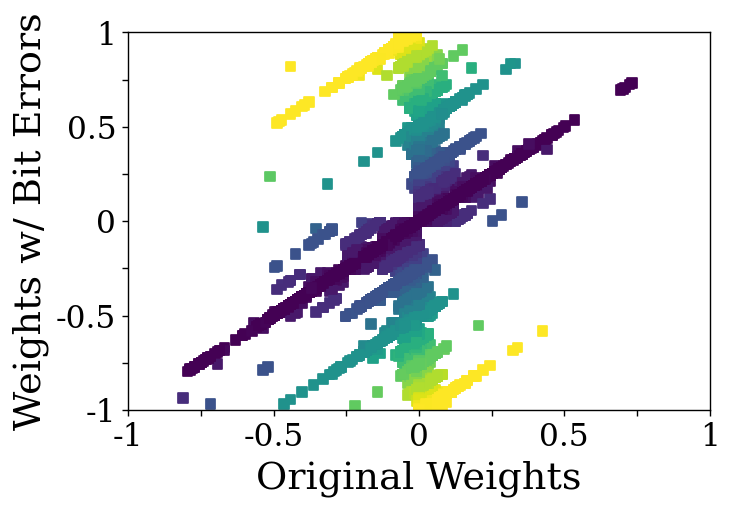
\includegraphics[height=3cm]{../paper/c10_errors_q81unfp_nt.png}};
						\node[anchor=north west] at (4,0){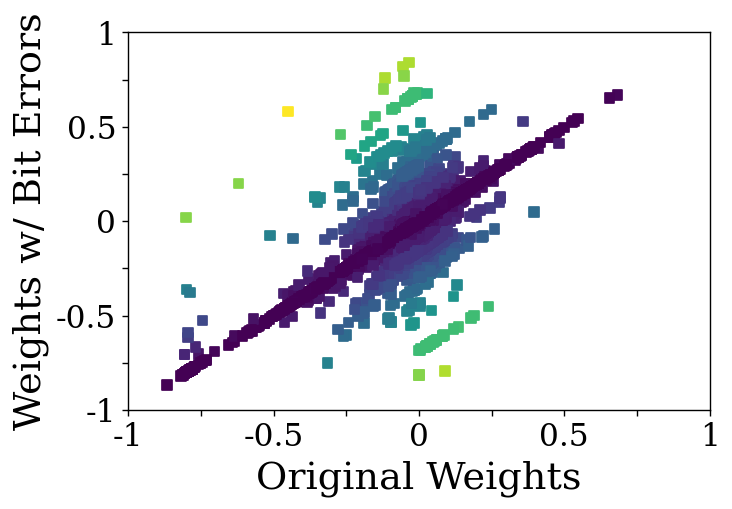
\includegraphics[height=3cm,trim=1cm 0 0 0,clip]{../paper/c10_errors_q81aunfp_nt.png}};
						\node[anchor=north west] at (8,0){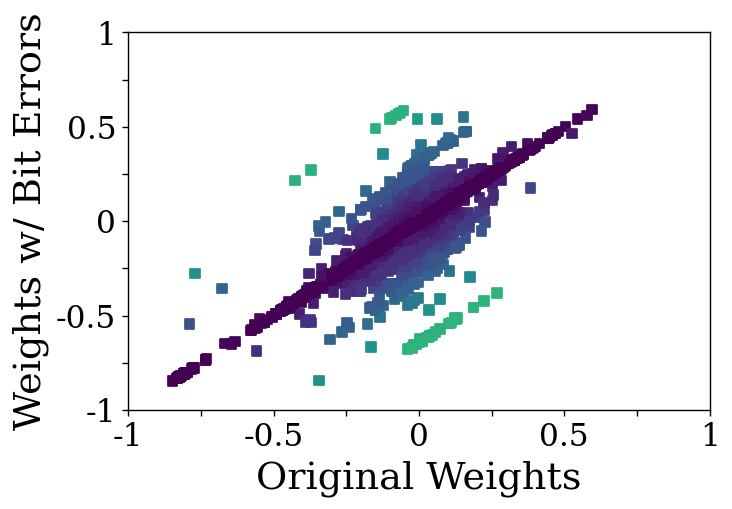
\includegraphics[height=3cm,trim=1cm 0 0 0,clip]{../paper/c10_errors_q81auunfp_nt.png}};
						
						\node[anchor=south,xshift=0.25cm,yshift=-0.25cm] at (2, 0){\textbf{Global}, $q_{\text{max}}=1$};
						\node[anchor=south,xshift=0.25cm,yshift=-0.25cm] at (6, 0){\textbf{Per-Layer}};
						\node[anchor=south,xshift=0.25cm,yshift=-0.25cm] at (10, 0){\textbf{{\color{red}+}Asymmetric}};
					\end{tikzpicture} 
				}
			\end{center}
		\end{tcolorbox}
	\end{frame}
	
	\begin{frame}[t]{\bfseries Robust Quantization (\textsc{RQuant})}
		\Large
		
		Simple fixed-point quantization scheme:
		\begin{align*}
			Q(w_i) = \left\lfloor\frac{w_i}{\Delta}\right\rfloor, Q^{-1}(v_i) = \Delta v_i, \Delta = \frac{q_{\text{max}}}{w^{m - 1} - 1}\notag
		\end{align*}
		\vspace*{-0.5cm}
		Importance of \textbf{implementation details}:
		\vspace*{0.3cm}
		\begin{center}
			\begin{tabular}{| c | l | c | c |}
				\hline
				\multicolumn{2}{|c|}{Quantization Scheme} & \multirow{2}{*}{\begin{tabular}{@{}c@{}}Err\\in \%\end{tabular}} & \multirow{2}{*}{\begin{tabular}{@{}c@{}}RErr\\in \%\end{tabular}}\\
				\multicolumn{2}{|c|}{(CIFAR-10, BER $p = 0.5\%$)} &&\\
				\hline
				\hline
				\multirow{4}{*}{\rotatebox{90}{$8$ bit}} & Per-layer & 4.36 & 24.76\\
				& +asymmetric & 4.36 & {\color{colorbrewer1}40.78}\\
				& +unsigned & 4.42 & 17.00\\
				& +rounding (=\textsc{RQuant}) & 4.32 & \bfseries 11.28\\
				\hline
			\end{tabular}
		\end{center}
	\end{frame}
	
	\begin{frame}[t]{\bfseries Robust Quantization (\textsc{RQuant})}
		\Large
		
		Simple fixed-point quantization scheme:
		\begin{align*}
			Q(w_i) = {\color{colorbrewer1}\left\lfloor\frac{w_i}{\Delta}\right\rceil}, Q^{-1}(v_i) = \Delta v_i, \Delta = \frac{q_{\text{max}}}{w^{m - 1} - 1}\notag
		\end{align*}
		\vspace*{-0.5cm}
		Importance of \textbf{implementation details}:
		\vspace*{0.3cm}
		\begin{center}
			\begin{tabular}{| c | l | c | c |}
				\hline
				\multicolumn{2}{|c|}{Quantization Scheme} & \multirow{2}{*}{\begin{tabular}{@{}c@{}}Err\\in \%\end{tabular}} & \multirow{2}{*}{\begin{tabular}{@{}c@{}}RErr\\in \%\end{tabular}}\\
				\multicolumn{2}{|c|}{(CIFAR-10, BER $p = 0.5\%$)} &&\\
				\hline
				\hline
				\multirow{2}{*}{\rotatebox{90}{$4$ bit}} & w/o rounding* & 5.81 & 90.36\\
				& w/ rounding* & \bfseries 5.29 & \bfseries 7.71\\
				\hline
				\multicolumn{4}{l}{\small *Results with weight clipping.}
			\end{tabular}
		\end{center}
	\end{frame}
	
	\begin{frame}[t]{\bfseries Robust Quantization (\textsc{RQuant})}
		\vspace*{0.25cm}
		\centering
		\hspace*{-1.6cm}
		\begin{tikzpicture}
		\begin{axis}[
				ymin=4.3,
				ymax=8,
				xmin=0,
				xmax=3,
				xtick={0, 0.01, 0.05, 0.1, 0.5, 1, 2.5},
				xticklabels={$0$, $0.01$, $0.05$, $0.1$, $0.5$, $1$, $2.5$},
				ytick={4.3, 5, 6, 7, 8, 9, 10},
				scaled x ticks=false,
				xticklabel style={/pgf/number format/precision=2,/pgf/number format/fixed},
				scaled y ticks=false,
				yticklabel style={/pgf/number format/precision=2,/pgf/number format/fixed},
				log ticks with fixed point,
				grid=major,
				xlabel={Bit Error Rate $p$ in \%},
				ylabel={Robust Test Error RErr in \%},
				x label style={at={(axis description cs:0.5,0.02)},anchor=north,font=\large},
				y label style={at={(axis description cs:0.07,0.5)},anchor=south,font=\large},
				width=10cm,
				height=7cm,
				legend style={at={(axis description cs:0.02,0.98)},anchor=north west,font=\small,fill opacity=0.4,text opacity=1},
				legend cell align={left},
			]
			
			\addplot[OptNormal] coordinates {
			(0.0, 4.36) % 0.0
			(0.005, 4.71) % 0.005
			(0.01, 4.82) % 0.01
			(0.025, 5.09) % 0.025
			(0.05, 5.510000000000001) % 0.05
			(0.075, 5.949999999999999) % 0.075
			(0.1, 6.370000000000001) % 0.1
			(0.25, 10.190000000000001) % 0.25
			(0.5, 24.759999999999998) % 0.5
			(0.75, 50.1) % 0.75
			(1.0, 72.65) % 1.0
			(1.5, 87.4) % 1.5
			(2.0, 89.75999999999999) % 2.0
			(2.5, 90.14999999999999) % 2.5
			};
			\label{normal1}
			\addplot[OptQuant] coordinates {
			(0.0, 4.32)
			(0.005, 4.52)
			(0.01, 4.6)
			(0.025, 4.83)
			(0.05, 5.1)
			(0.075, 5.3100000000000005)
			(0.1, 5.54)
			(0.25, 7.08)
			(0.5, 11.28)
			(0.75, 18.44)
			(1.0, 32.05)
			(1.5, 68.65)
			(2.0, 85.28)
			(2.5, 89.01)
			};
			\label{quant1}
			\end{axis}
			\node [draw,fill=white,text opacity=1,fill opacity=0.5,anchor=north west] at (rel axis cs: 0.02, 0.98) {\shortstack[l]{
			\underline{$8$ Bit Quant. CIFAR-10:}\\
			\ref{normal1} \textsc{Normal}\\[1px]
			\ref{quant1} \textsc{RQuant}}};
		\end{tikzpicture}
	\end{frame}
	
	\begin{frame}[t]{\bfseries Weight Clipping as Regularization (\textsc{Clipping})}
		\Large
	
		= clipping weights to $[-w_{\text{max}}, w_{\text{max}}]$ during training.
		\vspace*{0.2cm}
		
		Important:
		\begin{itemize}
			\item $w_{\text{max}} \neq q_{\text{max}}$, but $q_{\text{max}} \leq w_{\text{max}}$
			\item Does \emph{not} impact \emph{relative} errors!
		\end{itemize}
	\end{frame}
	
	\begin{frame}[t]{\bfseries Weight Clipping as Regularization (\textsc{Clipping})}
		\Large
	
		= clipping weights to $[-q_{\text{max}}, w_{\text{max}}]$ during training.
		\vspace*{0.2cm}
		
		Important:
		\begin{itemize}
			\item $w_{\text{max}} \neq q_{\text{max}}$, but $q_{\text{max}} \leq w_{\text{max}}$
			\item Does \emph{not} impact \emph{relative} errors!
		\end{itemize}
		
		\begin{tcolorbox}[
			enhanced,
			boxsep=0pt,
			left=5pt,
			right=5pt,
			top=0pt,
			toptitle=4pt,
			bottomtitle=2pt,
			bottom=0pt,
			colback=white,
			colframe=gray!12!white,
			width=1\textwidth, 
			enlarge left by=0mm,
			arc=0pt,outer arc=0pt,
			boxrule=1pt,
			title=,
			coltitle=MPIIblack,
			colbacktitle=gray!12!white,
			titlerule style=gray!12!white,
			collower=MPIIblack,
			]
			\begin{center}
				\hspace*{-0.4cm}
				\begin{minipage}[t]{0.48\textwidth}
					\vspace*{3px}
					
					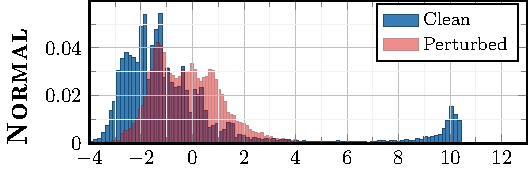
\includegraphics[height=1.75cm]{../paper/c10_q81auunfp_nt_original_logits.pdf}
				\end{minipage}
				\begin{minipage}[t]{0.24\textwidth}
					\vspace*{0px}
					
					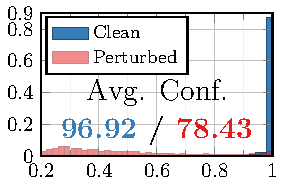
\includegraphics[height=1.75cm]{../paper/c10_q81auunfp_nt_original_confidences.pdf}
				\end{minipage}
				\begin{minipage}[t]{0.24\textwidth}
					\vspace*{0px}
					
					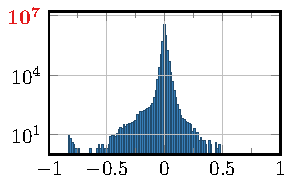
\includegraphics[height=1.75cm]{../paper/c10_q81auunfp_nt_original_weights.pdf}
				\end{minipage}
				
				\hspace*{-0.4cm}
				\begin{minipage}[t]{0.48\textwidth}
					\vspace*{3px}
					
					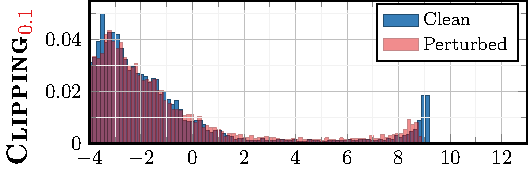
\includegraphics[height=1.75cm]{../paper/c10_q801auunfp_nt_original_logits.pdf}
				\end{minipage}
				\begin{minipage}[t]{0.24\textwidth}
					\vspace*{0px}
					
					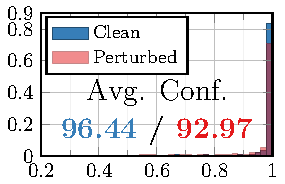
\includegraphics[height=1.75cm]{../paper/c10_q801auunfp_nt_original_confidences.pdf}
				\end{minipage}
				\begin{minipage}[t]{0.24\textwidth}
					\vspace*{0px}
					
					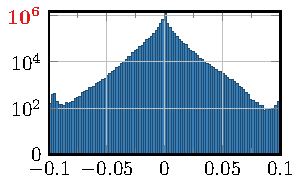
\includegraphics[height=1.75cm]{../paper/c10_q801auunfp_nt_original_weights.pdf}
				\end{minipage}
			\end{center}
		\end{tcolorbox}
	\end{frame}
	
	\begin{frame}[t]{\bfseries Weight Clipping as Regularization (\textsc{Clipping})}
		\Large
	
		\textbf{Why} does \textsc{Clipping} improve bit error robustness?
		
		\begin{itemize}
			\item Limiting weights and minimizing cross-entropy loss
			\item Large logits achievable through weight redundancy
		\end{itemize}
		
		\begin{center}
			\begin{tabular}{| l | c | c |}
				\hline
				Model & \multirow{2}{*}{\begin{tabular}{@{}c@{}}Err\\in \%\end{tabular}} & \multirow{2}{*}{\begin{tabular}{@{}c@{}}RErr\\in \%\end{tabular}}\\
				(CIFAR-10, BER $p{=}1\%$) &&\\
				\hline 
				\hline
				\textsc{RQuant} & \bfseries 4.32 & 32.05\\
				\hline
				\textsc{Clipping}\textsubscript{$0.15$} & 4.42 & 13.08\\
				\textsc{Clipping}\textsubscript{$0.15$}+label smoothing & 4.67 & {\color{colorbrewer1}29.40}\\
				\hline
			\end{tabular}
		\end{center}
	\end{frame}
	 
	\begin{frame}[t]{\bfseries Weight Clipping as Regularization (\textsc{Clipping})}
		\vspace*{0.25cm}
		\centering
		\hspace*{-1.6cm}
		\begin{tikzpicture}
		\begin{axis}[
				ymin=4.3,
				ymax=8,
				xmin=0,
				xmax=3,
				xtick={0, 0.01, 0.05, 0.1, 0.5, 1, 2.5},
				xticklabels={$0$, $0.01$, $0.05$, $0.1$, $0.5$, $1$, $2.5$},
				ytick={4.3, 5, 6, 7, 8, 9, 10},
				scaled x ticks=false,
				xticklabel style={/pgf/number format/precision=2,/pgf/number format/fixed},
				scaled y ticks=false,
				yticklabel style={/pgf/number format/precision=2,/pgf/number format/fixed},
				log ticks with fixed point,
				grid=major,
				xlabel={Bit Error Rate $p$ in \%},
				ylabel={Robust Test Error RErr in \%},
				x label style={at={(axis description cs:0.5,0.02)},anchor=north,font=\large},
				y label style={at={(axis description cs:0.07,0.5)},anchor=south,font=\large},
				width=10cm,
				height=7cm,
				legend style={at={(axis description cs:0.02,0.98)},anchor=north west,font=\small,fill opacity=0.4,text opacity=1},
				legend cell align={left},
			]
			
			\addplot[OptNormal] coordinates {
			(0.0, 4.36) % 0.0
			(0.005, 4.71) % 0.005
			(0.01, 4.82) % 0.01
			(0.025, 5.09) % 0.025
			(0.05, 5.510000000000001) % 0.05
			(0.075, 5.949999999999999) % 0.075
			(0.1, 6.370000000000001) % 0.1
			(0.25, 10.190000000000001) % 0.25
			(0.5, 24.759999999999998) % 0.5
			(0.75, 50.1) % 0.75
			(1.0, 72.65) % 1.0
			(1.5, 87.4) % 1.5
			(2.0, 89.75999999999999) % 2.0
			(2.5, 90.14999999999999) % 2.5
			};
			\label{normal1}
			\addplot[OptQuant] coordinates {
			(0.0, 4.32)
			(0.005, 4.52)
			(0.01, 4.6)
			(0.025, 4.83)
			(0.05, 5.1)
			(0.075, 5.3100000000000005)
			(0.1, 5.54)
			(0.25, 7.08)
			(0.5, 11.28)
			(0.75, 18.44)
			(1.0, 32.05)
			(1.5, 68.65)
			(2.0, 85.28)
			(2.5, 89.01)
			};
			\label{quant1}
			\addplot[OptClipping] coordinates {
			(0.0, 4.42)
			(0.005, 4.569999999999999)
			(0.01, 4.66)
			(0.025, 4.81)
			(0.05, 5.01)
			(0.075, 5.16)
			(0.1, 5.3100000000000005)
			(0.25, 6.17)
			(0.5, 6.529999999999999)
			(0.75, 6.8500000000000005)
			(1.0, 7.180000000000001)
			(1.5, 7.920000000000001)
			(2.0, 8.7)
			(2.5, 9.02)
			};
			\label{clipping1}
			\end{axis}
			\node [draw,fill=white,text opacity=1,fill opacity=0.5,anchor=north west] at (rel axis cs: 0.02, 0.98) {\shortstack[l]{
			\underline{$8$ Bit Quant.:}\\
			\ref{normal1} \textsc{Normal}\\[1px]
			\ref{quant1} \textsc{RQuant}\\
			\ref{clipping1} +\textsc{Clipping}}};
		\end{tikzpicture}
	\end{frame}
	
	\begin{frame}[t]{\bfseries Random bit error training (\textsc{RandBET})}
		\Large 
		= training on \emph{random} bit errors
		
		\begin{center}
			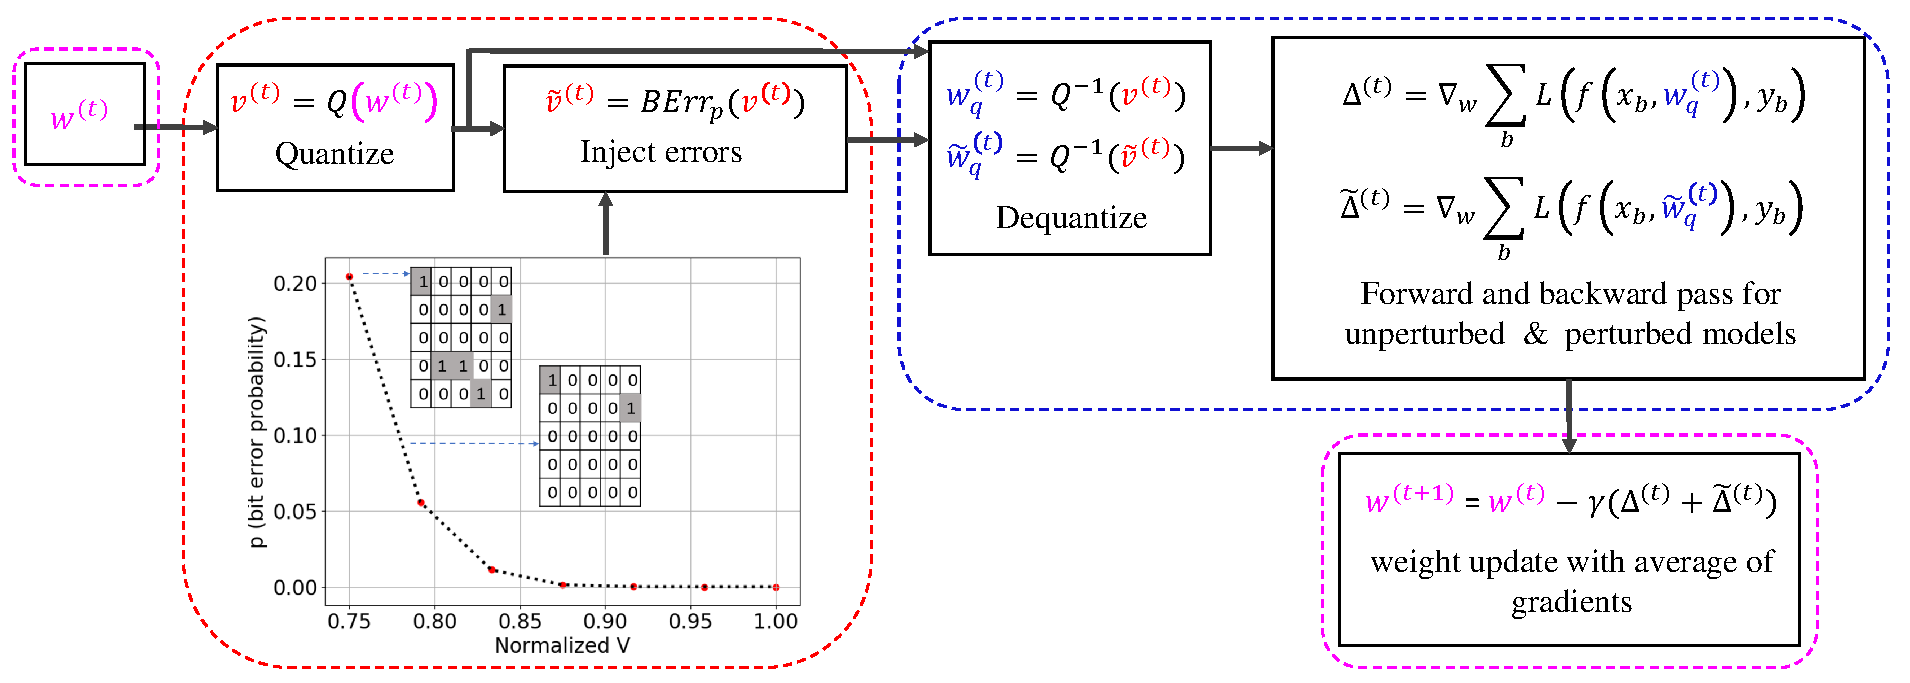
\includegraphics[width=\textwidth]{../paper/main_training_flow4}
		\end{center}
	\end{frame}
	
	\begin{frame}[t]{\bfseries Random bit error training (\textsc{RandBET})}
		\Large
		Important: train on \emph{random} bit errors.
		\vspace*{0.25cm}
		
		Related work frequently trains on \emph{profiled} bit errors.\\
		{\large(Specific to \emph{one} chip \emph{and} voltage.)}
		 
		\begin{center}
			\begin{tabular}{| l | c | c |}
				\hline
				Model & \multicolumn{2}{c|}{\RTE in \%, $p$ in \%}\\
				\hline
				\hline
				\textbf{Evaluation on Fixed Pattern} & $p{=}1$ & $p{=}2.5$\\
				\hline
				Fixed Pattern $p{=}2.5$ & {\color{colorbrewer1}14.14} & 7.87\\
				Fixed Pattern+\textsc{Clipping}\textsubscript{$0.15$} $p{=}2.5$ & {\color{colorbrewer1}8.50} & 7.41\\
				\hline\hline
				\textbf{Evaluation on \emph{Random} Patterns} & $p{=}1$ & $p{=}2.5$\\
				\hline
				Fixed Pattern+\textsc{Clipping}\textsubscript{$0.15$} $p{=}2.5$ & 12.09 & 61.59\\
				\hline
			\end{tabular}
		\end{center}
	\end{frame}
	
	\begin{frame}[t]{\bfseries Random bit error training (\textsc{RandBET})}
		\vspace*{0.25cm}
		\centering
		\hspace*{-1.6cm}
		\begin{tikzpicture}
		\begin{axis}[
				ymin=4.3,
				ymax=8,
				xmin=0,
				xmax=3,
				xtick={0, 0.01, 0.05, 0.1, 0.5, 1, 2.5},
				xticklabels={$0$, $0.01$, $0.05$, $0.1$, $0.5$, $1$, $2.5$},
				ytick={4.3, 5, 6, 7, 8, 9, 10},
				scaled x ticks=false,
				xticklabel style={/pgf/number format/precision=2,/pgf/number format/fixed},
				scaled y ticks=false,
				yticklabel style={/pgf/number format/precision=2,/pgf/number format/fixed},
				log ticks with fixed point,
				grid=major,
				xlabel={Bit Error Rate $p$ in \%},
				ylabel={Robust Test Error RErr in \%},
				x label style={at={(axis description cs:0.5,0.02)},anchor=north,font=\large},
				y label style={at={(axis description cs:0.07,0.5)},anchor=south,font=\large},
				width=10cm,
				height=7cm,
				legend style={at={(axis description cs:0.02,0.98)},anchor=north west,font=\small,fill opacity=0.4,text opacity=1},
				legend cell align={left},
			]
			
			\addplot[OptNormal] coordinates {
			(0.0, 4.36) % 0.0
			(0.005, 4.71) % 0.005
			(0.01, 4.82) % 0.01
			(0.025, 5.09) % 0.025
			(0.05, 5.510000000000001) % 0.05
			(0.075, 5.949999999999999) % 0.075
			(0.1, 6.370000000000001) % 0.1
			(0.25, 10.190000000000001) % 0.25
			(0.5, 24.759999999999998) % 0.5
			(0.75, 50.1) % 0.75
			(1.0, 72.65) % 1.0
			(1.5, 87.4) % 1.5
			(2.0, 89.75999999999999) % 2.0
			(2.5, 90.14999999999999) % 2.5
			};
			\label{normal1}
			\addplot[OptQuant] coordinates {
			(0.0, 4.32)
			(0.005, 4.52)
			(0.01, 4.6)
			(0.025, 4.83)
			(0.05, 5.1)
			(0.075, 5.3100000000000005)
			(0.1, 5.54)
			(0.25, 7.08)
			(0.5, 11.28)
			(0.75, 18.44)
			(1.0, 32.05)
			(1.5, 68.65)
			(2.0, 85.28)
			(2.5, 89.01)
			};
			\label{quant1}
			\addplot[OptClipping] coordinates {
			(0.0, 4.42)
			(0.005, 4.569999999999999)
			(0.01, 4.66)
			(0.025, 4.81)
			(0.05, 5.01)
			(0.075, 5.16)
			(0.1, 5.3100000000000005)
			(0.25, 6.17)
			(0.5, 6.529999999999999)
			(0.75, 6.8500000000000005)
			(1.0, 7.180000000000001)
			(1.5, 7.920000000000001)
			(2.0, 8.7)
			(2.5, 9.02)
			};
			\label{clipping1}
			\addplot[OptRandom] coordinates {
			(0.0, 4.44)
			(0.005, 4.65)
			(0.01, 4.67)
			(0.025, 4.8500000000000005)
			(0.05, 5.07)
			(0.075, 5.24)
			(0.1, 5.37)
			(0.25, 5.81)
			(0.5, 6.18)
			(0.75, 6.47)
			(1.0, 6.710000000000001)
			(1.5, 7.13)
			(2.0, 7.580000000000001)
			(2.5, 8.02)
			};
			\label{random1}
			\end{axis}
			\node [draw,fill=white,text opacity=1,fill opacity=0.5,anchor=north west] at (rel axis cs: 0.02, 0.98) {\shortstack[l]{
			\underline{$8$ Bit Quant.:}\\
			\ref{normal1} \textsc{Normal}\\[1px]
			\ref{quant1} \textsc{RQuant}\\
			\ref{clipping1} +\textsc{Clipping}\\[1px]
			\ref{random1} +\textsc{RandBET}}};
		\end{tikzpicture}
	\end{frame}
	
	\begin{frame}[t]{\bfseries Random bit error training (\textsc{RandBET})}
		\vspace*{0.25cm}
		\centering
		\hspace*{-1.6cm}
		\begin{tikzpicture}
		\begin{axis}[
				ymin=4.3,
				ymax=8,
				xmin=0,
				xmax=3,
				xtick={0, 0.01, 0.05, 0.1, 0.5, 1, 2.5},
				xticklabels={$0$, $0.01$, $0.05$, $0.1$, $0.5$, $1$, $2.5$},
				ytick={4.3, 5, 6, 7, 8, 9, 10},
				scaled x ticks=false,
				xticklabel style={/pgf/number format/precision=2,/pgf/number format/fixed},
				scaled y ticks=false,
				yticklabel style={/pgf/number format/precision=2,/pgf/number format/fixed},
				log ticks with fixed point,
				grid=major,
				xlabel={Bit Error Rate $p$ in \%},
				ylabel={Robust Test Error RErr in \%},
				x label style={at={(axis description cs:0.5,0.02)},anchor=north,font=\large},
				y label style={at={(axis description cs:0.07,0.5)},anchor=south,font=\large},
				width=10cm,
				height=7cm,
				legend style={at={(axis description cs:0.02,0.98)},anchor=north west,font=\small,fill opacity=0.4,text opacity=1},
				legend cell align={left},
			]
			
			\addplot[OptNormal] coordinates {
			(0.0, 4.36) % 0.0
			(0.005, 4.71) % 0.005
			(0.01, 4.82) % 0.01
			(0.025, 5.09) % 0.025
			(0.05, 5.510000000000001) % 0.05
			(0.075, 5.949999999999999) % 0.075
			(0.1, 6.370000000000001) % 0.1
			(0.25, 10.190000000000001) % 0.25
			(0.5, 24.759999999999998) % 0.5
			(0.75, 50.1) % 0.75
			(1.0, 72.65) % 1.0
			(1.5, 87.4) % 1.5
			(2.0, 89.75999999999999) % 2.0
			(2.5, 90.14999999999999) % 2.5
			};
			\label{normal1}
			\addplot[OptQuant] coordinates {
			(0.0, 4.32)
			(0.005, 4.52)
			(0.01, 4.6)
			(0.025, 4.83)
			(0.05, 5.1)
			(0.075, 5.3100000000000005)
			(0.1, 5.54)
			(0.25, 7.08)
			(0.5, 11.28)
			(0.75, 18.44)
			(1.0, 32.05)
			(1.5, 68.65)
			(2.0, 85.28)
			(2.5, 89.01)
			};
			\label{quant1}
			\addplot[OptClipping] coordinates {
			(0.0, 4.42)
			(0.005, 4.569999999999999)
			(0.01, 4.66)
			(0.025, 4.81)
			(0.05, 5.01)
			(0.075, 5.16)
			(0.1, 5.3100000000000005)
			(0.25, 6.17)
			(0.5, 6.529999999999999)
			(0.75, 6.8500000000000005)
			(1.0, 7.180000000000001)
			(1.5, 7.920000000000001)
			(2.0, 8.7)
			(2.5, 9.02)
			};
			\label{clipping1}
			\addplot[OptRandom] coordinates {
			(0.0, 4.44)
			(0.005, 4.65)
			(0.01, 4.67)
			(0.025, 4.8500000000000005)
			(0.05, 5.07)
			(0.075, 5.24)
			(0.1, 5.37)
			(0.25, 5.81)
			(0.5, 6.18)
			(0.75, 6.47)
			(1.0, 6.710000000000001)
			(1.5, 7.13)
			(2.0, 7.580000000000001)
			(2.5, 8.02)
			};
			\label{random1}
			\coordinate (e) at (axis cs:0.5,6.18);
			\coordinate (e2) at (axis cs:0.1,5.37);
			\end{axis}
			\draw[colorbrewer1,line width=2pt] (e) circle (6pt);
			\draw[colorbrewer1,line width=2pt,-] ($(e) - (0,0.2)$) -- ($(e) - (0,2.9)$);
			\draw[colorbrewer1,line width=2pt,-] ($(e) - (0.2,0)$) -- ($(e) - (6.9,0)$);
			\node[opacity=1,fill opacity=0.75,fill=white] at ($(e) - (4.25,0)$){\bfseries\color{colorbrewer1}$\mathbf{6.18\%}$ ${\approx}$ $\mathbf{30\%}$ reduction};
			
			\draw[colorbrewer1,line width=2pt] (e2) circle (6pt);
			\draw[colorbrewer1,line width=2pt,-] ($(e2) - (0,0.2)$) -- ($(e2) - (0,1.7)$);
			\draw[colorbrewer1,line width=2pt,-] ($(e2) - (0.2,0)$) -- ($(e2) - (5.35,0)$);
			\node[opacity=1,fill opacity=0.75,fill=white] at ($(e2) - (2.75,0)$){\bfseries\color{colorbrewer1}$\mathbf{5.37\%}$ ${\approx}$ $\mathbf{20\%}$ reduction};
			
			\node [draw,fill=white,text opacity=1,fill opacity=0.5,anchor=north west] at (rel axis cs: 0.02, 0.98) {\shortstack[l]{
			\underline{$8$ Bit Quant.:}\\
			\ref{normal1} \textsc{Normal}\\[1px]
			\ref{quant1} \textsc{RQuant}\\ 
			\ref{clipping1} +\textsc{Clipping}\\[1px]
			\ref{random1} +\textsc{RandBET}}};
		\end{tikzpicture}
	\end{frame}
	
	\begin{frame}[t]{\bfseries Low-Voltage \emph{and} Low-Precision}
		\vspace*{0.25cm}
		\centering
		\hspace*{-1.6cm}
		\begin{tikzpicture}
		\begin{axis}[
				ymin=4.3,
				ymax=8,
				xmin=0,
				xmax=3,
				xtick={0, 0.01, 0.05, 0.1, 0.5, 1, 2.5},
				xticklabels={$0$, $0.01$, $0.05$, $0.1$, $0.5$, $1$, $2.5$},
				ytick={4.3, 5, 6, 7, 8, 9, 10},
				scaled x ticks=false,
				xticklabel style={/pgf/number format/precision=2,/pgf/number format/fixed},
				scaled y ticks=false,
				yticklabel style={/pgf/number format/precision=2,/pgf/number format/fixed},
				log ticks with fixed point,
				grid=major,
				xlabel={Bit Error Rate $p$ in \%},
				ylabel={Robust Test Error RErr in \%},
				x label style={at={(axis description cs:0.5,0.02)},anchor=north,font=\large},
				y label style={at={(axis description cs:0.07,0.5)},anchor=south,font=\large},
				width=10cm,
				height=7cm,
				legend style={at={(axis description cs:0.02,0.98)},anchor=north west,font=\small,fill opacity=0.4,text opacity=1},
				legend cell align={left},
			]
			
			\addplot[OptNormal,opacity=0.25,mark options={opacity=0.25,fill opacity=0.25}] coordinates {
			(0.0, 4.36) % 0.0
			(0.005, 4.71) % 0.005
			(0.01, 4.82) % 0.01
			(0.025, 5.09) % 0.025
			(0.05, 5.510000000000001) % 0.05
			(0.075, 5.949999999999999) % 0.075
			(0.1, 6.370000000000001) % 0.1
			(0.25, 10.190000000000001) % 0.25
			(0.5, 24.759999999999998) % 0.5
			(0.75, 50.1) % 0.75
			(1.0, 72.65) % 1.0
			(1.5, 87.4) % 1.5
			(2.0, 89.75999999999999) % 2.0
			(2.5, 90.14999999999999) % 2.5
			};
			\label{normal}
			\addplot[OptQuant,opacity=0.25,mark options={opacity=0.25,fill opacity=0.25}] coordinates {
			(0.0, 4.32)
			(0.005, 4.52)
			(0.01, 4.6)
			(0.025, 4.83)
			(0.05, 5.1)
			(0.075, 5.3100000000000005)
			(0.1, 5.54)
			(0.25, 7.08)
			(0.5, 11.28)
			(0.75, 18.44)
			(1.0, 32.05)
			(1.5, 68.65)
			(2.0, 85.28)
			(2.5, 89.01)
			};
			\label{quant}
			\addplot[OptClipping,opacity=0.25,mark options={opacity=0.25,fill opacity=0.25}] coordinates {
			(0.0, 4.42)
			(0.005, 4.569999999999999)
			(0.01, 4.66)
			(0.025, 4.81)
			(0.05, 5.01)
			(0.075, 5.16)
			(0.1, 5.3100000000000005)
			(0.25, 6.17)
			(0.5, 6.529999999999999)
			(0.75, 6.8500000000000005)
			(1.0, 7.180000000000001)
			(1.5, 7.920000000000001)
			(2.0, 8.7)
			(2.5, 9.02)
			};
			\label{clipping}
			\addplot[OptRandom,opacity=0.25,mark options={opacity=0.25,fill opacity=0.25}] coordinates {
			(0.0, 4.44)
			(0.005, 4.65)
			(0.01, 4.67)
			(0.025, 4.8500000000000005)
			(0.05, 5.07)
			(0.075, 5.24)
			(0.1, 5.37)
			(0.25, 5.81)
			(0.5, 6.18)
			(0.75, 6.47)
			(1.0, 6.710000000000001)
			(1.5, 7.13)
			(2.0, 7.580000000000001)
			(2.5, 8.02)
			};
			\label{random}
			\addplot[Opt] coordinates {
			(0.0, 4.32)
			(0.005, 4.52)
			(0.01, 4.6)
			(0.025, 4.81)
			(0.05, 5.01)
			(0.075, 5.16)
			(0.1, 5.3100000000000005)
			(0.25, 5.81)
			(0.5, 6.18)
			(0.75, 6.47)
			(1.0, 6.710000000000001)
			(1.5, 7.13)
			(2.0, 7.580000000000001)
			(2.5, 8.02)
			};
			\label{opt}
			\addplot[Opt2] coordinates {
			(0.0, 4.5)
			(0.005, 4.65)
			(0.01, 4.72)
			(0.025, 4.89)
			(0.05, 5.050000000000001)
			(0.075, 5.220000000000001)
			(0.1, 5.36)
			(0.25, 5.94)
			(0.5, 6.38)
			(0.75, 6.68)
			(1.0, 6.98)
			(1.5, 7.51)
			(2.0, 8.06)
			(2.5, 8.62)
			};
			\label{opt2}
			\end{axis}
			\node [draw,fill=white,text opacity=1,fill opacity=0.5,anchor=north west] at (rel axis cs: 0.02, 0.98) {\shortstack[l]{
			\underline{$8$ Bit Quant.:}\\
			\ref{normal} \textsc{Normal}\\[1px]
			\ref{quant} \textsc{RQuant}\\
			\ref{clipping} +\textsc{Clipping}\\[1px]
			\ref{random} +\textsc{RandBET}}};
			\node [draw,fill=white,text opacity=1,fill opacity=0.5,anchor=south east] at (rel axis cs: 0.98, 0.02) {\shortstack[l]{
			\ref{opt} Best, $8$ bits\\
			\ref{opt2} Best, $4$ bits}};
		\end{tikzpicture}
	\end{frame}
	
	\begin{frame}[t]{\bfseries Generalization Across Chips/Voltages}
		\Large
		
		\begin{tikzpicture}
			\node[anchor=north west] at (-0.25,1.75){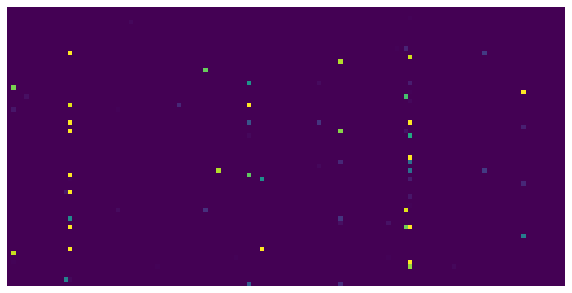
\includegraphics[width=6cm,trim={0 5cm 0 0},clip]{gfx/n_3}};
			\node[anchor=north west] at (5.75,1.75){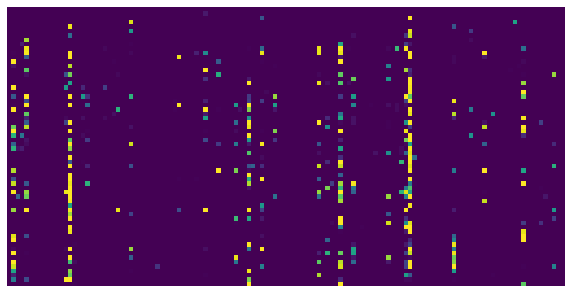
\includegraphics[width=6cm,trim={0 5cm 0 0},clip]{gfx/n_2}};
			\draw[line width=1pt,-] (2.75,-0.175) -- (2.75,-0.5) -- (4.5,-0.5);
			\draw[line width=1pt,-] (7,-0.5) -- (8.75,-0.5) -- (8.75,-0.175);
			\node at (5.75,-0.5){\normalsize subset of};
			\node[anchor=north west,fill=white,fill opacity=0.6,text opacity=1,inner sep=2.5pt] at (0.1, 1.4){\normalsize $p{\approx}0.14\%$};
			\node[anchor=north west,fill=white,fill opacity=0.6,text opacity=1,inner sep=2.5pt] at (6.1, 1.4){\normalsize $p{\approx}1.08\%$};
		\end{tikzpicture}
		
		\begin{itemize}
			\item ``Corner-cases'' might exhibit different error patterns.
		\end{itemize}
		
		\begin{center}
			\begin{tabular}{| l | l | c | c |}
				\hline
				Chip & Model (CIFAR-10)& \multicolumn{2}{c|}{\RTE in \%}\\
				\hline
				\hline
				\bfseries Chip 1 && $p{\approx}0.86$ & {\color{colorbrewer1}$p{\approx}2.75$}\\
				\hline
				& \textsc{RandBET}\textsubscript{$0.05$} $p{=}1.5$ & 7.04 & 9.37\\
				\hline
				\hline
				\bfseries Chip 2 & (see above) & $p{\approx}0.14$ & {\color{colorbrewer1}$p{\approx}1.08$}\\
				\hline
				& \textsc{RandBET}\textsubscript{$0.05$} $p{=}1.5$ & 6.00 & 9.00\\
				\hline
			\end{tabular}
		\end{center}
	\end{frame}
	
	\begin{frame}[t]{\bfseries Bit Error Robustness for DNN Accelerators}
		\Large
		
		\begin{tikzpicture}[overlay,remember picture]
			\node[anchor=north west] at (6,1){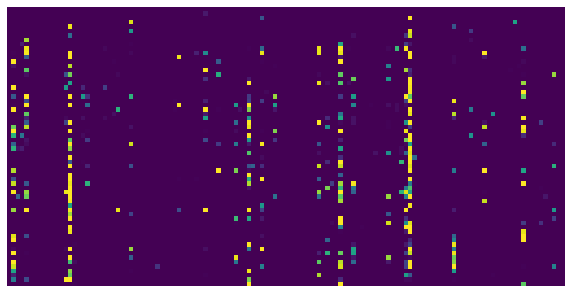
\includegraphics[width=6cm,trim={0 3cm 0 0},clip]{gfx/n_2}};
		\end{tikzpicture}
		
		\vspace*{-0.75cm}
		\underline{Conclusion:}
		\begin{itemize}
			\item Uniform bit error model.
			\item Robust quantization.
			\item Weight clipping and random bit error training.
			\item Generalization across chips and voltages.
		\end{itemize}
		
		\begin{paper}{}
			\underline{Paper:} \url{https://davidstutz.de/randbet}
			\begin{itemize}
				\item Results on MNIST / CIFAR-100, guarantees, ...
			\end{itemize}
		\end{paper}
	\end{frame}
\end{document}
